\section{Introduction}
This chapter looks at the historical relationship between the Papuan languages of Alor-Pantar (AP) and those of Timor-Kisar (TK). The TK group of Papuan languages consists of Bunaq\il{Bunaq}, spoken in central Timor; Makasae\il{Makasae}, Makalero\il{Makalero} and Fataluku\il{Fataluku}, three languages spoken in a contiguous region of far eastern Timor; and Oirata\il{Oirata}, spoken on the southern side of Kisar Island to the north of Timor. Due to their geographical proximity, AP and TK languages have typically been assumed to be related to one another (e.g., \citealt{Stokhof1975,Capell1975}). Together they have been referred to as the Timor-Alor-Pantar (TAP) family. However, there has been no substantive data-driven investigation of the claim of relatedness.

In this chapter, we test the hypothesis that AP and TK languages are related to one another through the application of the comparative method. Specifically, we compare the results of two recent reconstructions, the one of AP \citep{HoltonEtAl2012} and the other of TK \citep{SchapperEtAl2012}. We establish that the AP and TK languages are indeed related by demonstrating that there are regular sound correspondences across cognate vocabulary between the two groups. 

In comparing \citet{HoltonEtAl2012} and \citet{SchapperEtAl2012} in this chapter, we assume the existence of two nodes in the TAP tree, namely Proto-Alor-Pantar (pAP)\il{proto-Alor-Pantar} and Proto-Timor (pTIM)\il{proto-Timor}. Whilst pAP\il{proto-Alor-Pantar} appears to be a robust node, the existence of pTIM\il{proto-Timor} is less secure. As \citet[227-228]{SchapperEtAl2012} point out, it is possible that Bunaq\il{Bunaq} and the Eastern Timor languages (reconstructed as Proto-ET\il{proto-Eastern Timor} in \citealt{SchapperEtAl2012}) both form their own separate primary subgroups within TAP. Our aim here is not to make claims about the high-level subgrouping of the AP and TK languages, and we do not presume to definitively determine the constituency of the TK-AP tree at this stage, but merely seek to show that TK and AP languages are related. Conclusive evidence of innovations\is{innovation} shared by Bunaq\il{Bunaq} and ET languages to the exclusion of AP languages is the subject of ongoing research. 

% \begin{figure}
% 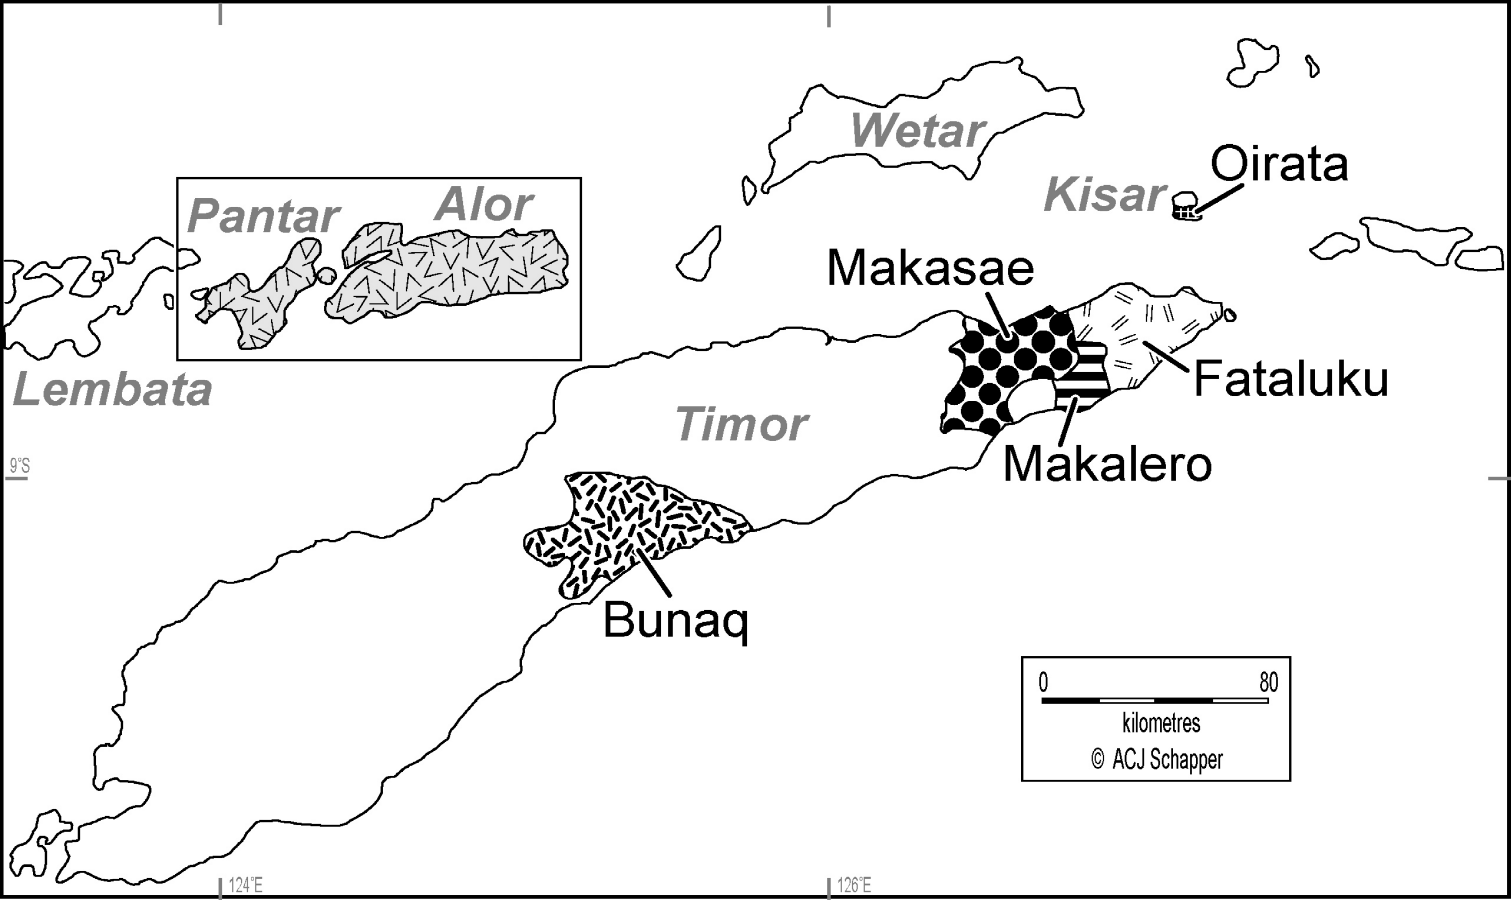
\includegraphics[width=\textwidth]{figures/ch3_map.png}
% \caption[The Papuan languages of Timor and Kisar]{The Papuan languages of Timor and Kisar. Hatching marks areas where Papuan languages are found. Only Timor-Kisar languages are marked by name}
% \end{figure}

\sectref{sec:3:2} presents the sound correspondences we find in cognate vocabulary between pAP\il{proto-Alor-Pantar} and pTIM\il{proto-Timor}. \sectref{sec:3:3} summarizes our preliminary findings and discusses issues arising out of them.  Appendices are included with supporting language data for any reconstructions that do not appear in \citet{HoltonEtAl2012} or \citet{SchapperEtAl2012}, as well as a list of pTAP\il{proto-Timor Alor Pantar} forms that can be reconstructed on the basis of the sound correspondences identified in this chapter. New, additional reconstructions have in some cases been necessary since the two articles each reconstruct only a small number of lexemes with only partial overlap between them.  The sources of the lexical data used are listed in the Appendices. We also throw out several cognate sets from the AP reconstruction as they reflect borrowing\is{borrowing} from Austronesian languages\il{Austronesian language(s)}. 

\section{Sound correspondences}\label{sec:3:2}
In this section, we describe the consonant correspondences that we have identified between AP and TK languages. We do draw on vowel correspondences where they condition particular sound changes in consonants, but otherwise do not deal with vowels in this preliminary demonstration of relatedness. We chiefly draw attention to the correspondences in cognate vocabulary between pAP\il{proto-Alor-Pantar} and pTIM\il{proto-Timor}. However, we provide the reader also with the forms of the lexemes in the TK languages as they are not available elsewhere in this volume. The argumentation and underpinning data for pAP\il{proto-Alor-Pantar} is given in \citet{HoltonRobinsonTVhistory} and is based on \citet{HoltonEtAl2012}.

In the subsections that follow, transcription of language data adheres to IPA conventions. Long vowels are indicated with a length mark `{\textlengthmark}'. Bracketed segments `( )' are those deemed to be non-etymological, that is, typically reflecting some morpheme which has fossilized on a root. In the correspondence tables, square brackets `[]' are used where an item is cognate but doesn't reflect the segment in question. The inverted question mark `?`' is used where a cognate shows an unexpected reflex of the segment in question. Grammatical items are glossed in small caps. Reconstructions marked with `!!' are new reconstructions not found in or revised from \citet{HoltonEtAl2012} or \citet{SchapperEtAl2012}. The symbol `!!' signals that the full data set on which the reconstruction in question is based is given in the Appendices. AP data supporting the additional pAP\il{proto-Alor-Pantar} reconstructions is given in Appendix \ref{sec:3:app:1} and TK data in Appendix \ref{sec:3:app:2}. In the text of the chapter itself, for reasons of compactness, we only give simple one-word glosses which reflect the presumed meaning of the proto-lexeme. Should the reader need more information on semantics, he can refer to the Appendices. We also do not provide information on irregular changes, such as metathesis\is{metathesis} or apocope\is{apocope}, in the correspondence tables, except where directly relevant to the reconstruction of the segment in question. The Appendix provides the reader with fuller information on any irregularities in form or meaning in individual languages. 

\subsection{Reconstruction of bilabial stops}
We identify two robust correspondent sets for bilabial plosives, reconstructing to pTAP\il{proto-Timor Alor Pantar} *p and *b. Note that in \citet{SchapperEtAl2012}, we reconstruct a three-way distinction (*p, *b, and *f) for bilabial obstruents in pTIM\il{proto-Timor}, despite the fact that it is not maintained in any of the modern TK languages: Bunaq\il{Bunaq}, Makasae\il{Makasae} and Makalero\il{Makalero} have merged reflexes of pTIM\il{proto-Timor} *p and *f, whereas in Fataluku\il{Fataluku} and Oirata\il{Oirata}, *p and *b are merged. We find no evidence to support a three-way split in pTAP\il{proto-Timor Alor Pantar}; instead, it looks like pTIM\il{proto-Timor} underwent a conditioned phoneme split, with distinct reflexes of pTAP\il{proto-Timor Alor Pantar} *b in initial and non-initial positions, respectively. 

\newpage 
Table~\ref{tab:3:1} and Table~\ref{tab:3:2} present the forms for these two correspondence sets respectively. In the first, pAP\il{proto-Alor-Pantar} *p corresponds to pTIM\il{proto-Timor} *f in all positions. In the second, pTAP\il{proto-Timor Alor Pantar} *b was retained as *b in pAP\il{proto-Alor-Pantar}, but split to pTIM\il{proto-Timor} *b initially and pTIM\il{proto-Timor} *p non-initially. In these sets, there are two notable irregularities: 
(i) pAP\il{proto-Alor-Pantar} *tiara `expel' lost the medial bilabial that is retained in pTIM\il{proto-Timor} *tifar `run'; and 
(ii) pAP\il{proto-Alor-Pantar} *karab `scratch' and pTIM\il{proto-Timor} *gabar `scratch', which show an irregular correspondence of pAP\il{proto-Alor-Pantar} *b with pTIM\il{proto-Timor} *b in medial position. 
 


\begin{sidewaystable}
\caption{Correspondence sets for pTAP\ilt{proto-Timor Alor Pantar} *p}
\label{tab:3:1}  
\begin{tabular*}{\textwidth}{llllllll}
\mytoprule
 & pAP\ilt{proto-Alor-Pantar} & pTIM\ilt{proto-Timor} & Bunaq\ilt{Bunaq} & Makasae\ilt{Makasae} & Makalero\ilt{Makalero} & Fataluku\ilt{Fataluku} & Oirata\ilt{Oirata}\\
\midrule
{\bfseries initial *p} & {\bfseries *p} & {\bfseries *f} & {\bfseries p, w} & {\bfseries f} & {\bfseries f} & {\bfseries f} & {\bfseries p}\\
spit & *purVn !! & *fulu(k, n) !! & {\itshape puluk} & -- & {\itshape fulun} & {\itshape fulu} & --\\
taboo & *palol !! & *falu(n) & \textit{por} & \textit{falun} & \textit{falun} & {\itshape falu} & --\\
1\textsc{pl} & *pi- & *fi & -- & \textit{fi} & \textit{fi} & \textit{afa} & \textit{ap}-\\
\textsc{low}\textsuperscript{1} & *po !! & *ufe !! & -- & \textit{he}- ?` & \textit{ufe}- & [\textit{ua}] & [\textit{ua}]\\
girl & *pon !! & *fana\textsuperscript{2} & \textit{pana} & \textit{fana(rae)} & \textit{fana(r)} & \textit{fana(r)} & \textit{pana(rai)}\\
scorpion & *pVr & *fe(r, R)e !! & \textit{wele} & -- & -- & -- & --\\
{\bfseries medial *p} & {\bfseries *p} & {\bfseries *f} & \textbf{w}, \textbf{{\O}} & {\bfseries f} & {\bfseries f} & {\bfseries f} & {\bfseries p}\\
face & *-pona !! & *-fanu !! & {}-\textit{ewen} & \textit{fanu} & \textit{fanu} & \textit{fanu} & \textit{panu}\\
dream & *hipar & *ufar(ana) !! & \textit{waen} & \textit{ufarena} & \textit{ofarana} & \textit{ufarana} & \textit{upar(a)}\\
run & [*tiara] & *tifar & \textit{t{\textesh}iwal} & [\textit{ditar}]& [\textit{titar}]& \textit{tifar}(\textit{e}) & \textit{tipar}(\textit{e})\\
pound & *tapai & *tafa & \textit{tao}\textsuperscript{3} & -- & \textit{tafa} & \textit{tafa} & \textit{tapa}\\
\mybottomrule
\end{tabular*}
 
\raggedright
\textsuperscript{1} This item is a deictic\ist{deixis} marker indicating lower elevation\ist{elevation} than the deictic\ist{deixis} center. See \citet{SchapperTVelevation} for more information on this deictic\ist{deixis} distinction.

\textsuperscript{2} The bracketed \textit{rae/r/rai} element appears to be an innovation\ist{innovation} in the Eastern Timor languages, presumably a lexical doublet or a derivational morpheme related to the nominalizing\ist{nominalization} \textit{{}-r} formative found in Makalero\ilt{Makalero}. We have no evidence for reconstructing this element higher than Proto-Eastern Timor\il{proto-Eastern Timor}.

\textsuperscript{3} This would have originally been *tawo in pre-Bunaq\ilt{Bunaq}, but in the modern language medial /w/ is not preserved before back vowels. 
\end{sidewaystable}

 

\begin{sidewaystable} 
\caption{Correspondence sets for pTAP\ilt{proto-Timor Alor Pantar} *b}
\label{tab:3:2} 
\begin{tabular*}{\textwidth}{llllllll}
\mytoprule
 & pAP\ilt{proto-Alor-Pantar} & pTIM\ilt{proto-Timor} & Bunaq\ilt{Bunaq} & Makasae\ilt{Makasae} & Makalero\ilt{Makalero} & Fataluku\ilt{Fataluku} & Oirata\ilt{Oirata}\\
\midrule
{\bfseries inital *b} & {\bfseries *b} & {\bfseries *b} & {\bfseries b} & {\bfseries b} & {\bfseries p} & {\bfseries p} & {\bfseries h}\\
pig & *baj & *baj & -- &{\itshape  baj} &{\itshape  paj} &{\itshape  paj} &{\itshape  haj}\\
price & *bol !! & *bura &{\itshape  bol} &{\itshape  bura} &{\itshape  pura} &{\itshape  pura} &{\itshape  hura}\\
mat & *bis & *biti !! & -- & -- &{\itshape  piti} &{\itshape  pet(u)} &{\itshape  het(e)}\\
leg & *-bat !! & *-buta !! & {\itshape {}-but} & -- & -- & -- & --\\
mountain & *buku !! & *bugu !! & -- & {\itshape bu{\textglotstop}u} & {\itshape{\itshape  pu{\textglotstop}u}} & -- & --\\
{\bfseries non-initial *b} & {\bfseries *b} & {\bfseries *p} & {\bfseries  p,  w} & {\bfseries f} & {\bfseries f} & {\bfseries p} & {\bfseries h}\\
fish & *habi !! & *hapi !! & -- &{\itshape  afi} &{\itshape  afi} &{\itshape  api} &{\itshape  ahi}\\
star & *jibV\textsuperscript{1} & *ipi(-bere) & [\textit{bi}]\textsuperscript{2} &{\itshape  ifi-bere} &{\itshape  ifi} &{\itshape  ipi(naka)} &{\itshape  ihi}\\
shark & *sib(a, i)r !!\textsuperscript{3} & *supor !! & -- & -- & [\textit{su}]\textsuperscript{4} &   \textit{hopor}(\textit{u}) & --\\
sugarcane & *huːba !! & *upa &{\itshape  up} &{\itshape  ufa} &{\itshape  ufa} &{\itshape  upa} &{\itshape  uha}\\
tongue & *-lebur !! & *-ipul &{\itshape  {}-up} &{\itshape  ifi} &{\itshape  ifil} &{\itshape  epul(u)} &{\itshape  uhul(u)}\\
dog & *jibar !!\textsuperscript{5} & *Depar &{\itshape  zap} &{\itshape  defa} &{\itshape  sefar} &{\itshape  ipar(u)} &{\itshape  ihar(a)}\\
other & *aben(VC) !! & *epi !! &{\itshape  ewi} & -- & -- & -- & --\\
scratch & *karab !! & *gabar ?` !!\textsuperscript{6} & -- & -- &{\itshape  kapar} &{\itshape  kafur(e)} & --\\
new & *siba(r) !! & *(t, s)ipa(r) ?` !! &{\itshape  tip} & {\itshape sufa} & {\itshape hofar} & -- & --\\
\mybottomrule
\end{tabular*}

 
\raggedright
\textsuperscript{1} Several AP languages have a compound for `star', although the second element does not appear to be cognate to that reconstructed for pTIM\ilt{proto-Timor}. Note also that \citet{HoltonEtAl2012} gave this item as *jibC.
% ; this error has been corrected for \citet{HoltonRobinsonTVhistory}.

\textsuperscript{2} The Bunaq\ilt{Bunaq} form reflects the second half of the pTIM\ilt{proto-Timor} doublet that is not found in AP languages.

\textsuperscript{3} The cognate set for this item is given in \citet{HoltonEtAl2012}, but no pAP\ilt{proto-Alor-Pantar} reconstruction is given.

\textsuperscript{4} The reflex of the relevant bilabial has been lost in Makalero\ilt{Makalero} due to apocope\ist{apocope}.

\textsuperscript{5} The cognate set for this item is given in \citet{HoltonEtAl2012}, but no pAP\ilt{proto-Alor-Pantar} reconstruction is given.

\textsuperscript{6} This form shows liquid-stop metathesis\ist{metathesis}. There is no evidence of *b occurring word-finally in pTIM\ilt{proto-Timor}.
\end{sidewaystable}



% At this stage, we have no evidence for the reconstruction of a third bilabial obstruent to pTAP\il{proto-Timor Alor Pantar}, as is found in pTIM\il{proto-Timor} (*p, *b and *f), but not pAP\il{proto-Alor-Pantar} (*p and*b). Based on the current correspondence sets, the three-way distinction appears to have arisen due to pTAP\il{proto-Timor Alor Pantar} medial *b changing to pTIM\il{proto-Timor} *p, while pTAP\il{proto-Timor Alor Pantar} *b stayed *b initially in pTIM\il{proto-Timor}. We are yet to find any AP cognates for words reconstructing with initial *p in pTIM\il{proto-Timor}.

\subsection{Reconstruction of coronal stops}
There are two coronal stops, *t and *d, reconstructed to pAP\il{proto-Alor-Pantar}, and four, *t, *d, *T and *D to pTIM\il{proto-Timor}. \citet{SchapperEtAl2012} note the uncertainty of pTIM\il{proto-Timor} *d, which is supported by three cognate sets only, all of which are in initial position. This is played out also when comparing coronals between AP and TK languages. We can reconstruct the pTAP\il{proto-Timor Alor Pantar} coronal stops *t with relative certainty, and *d, albeit with less security. The latter segment split in pTIM\il{proto-Timor} to *T and *D. At present, we cannot reconstruct pTIM\il{proto-Timor} *d to pTAP\il{proto-Timor Alor Pantar}. There are, however, a substantial number of coronal correspondences which remain unexplained. 

Our most consistent correspondence is pTIM\il{proto-Timor} *t to pAP\il{proto-Alor-Pantar} *t and *s (Table~\ref{tab:3:3}). Initially, we find a steady and unchanging correspondence of pAP\il{proto-Alor-Pantar} *t and pTIM\il{proto-Timor} *t, supported by a sizeable number of cognates. Only Bunaq\il{Bunaq} shows a change of *t to /t{\textesh}/ before a high front vowel. Non-initially, we find fewer cognates, but nevertheless a steady and unchanging correspondence. In two cognate sets (`sit' and `mat'), pAP\il{proto-Alor-Pantar} final *s preceded by *i corresponds to pTIM\il{proto-Timor} *t.
 

\begin{sidewaystable}
\caption{Correspondence sets for pTAP\ilt{proto-Timor Alor Pantar} *t}
\label{tab:3:3}  
\begin{tabular*}{\textwidth}{llllllll}
\mytoprule
 & pAP\ilt{proto-Alor-Pantar} & pTIM\ilt{proto-Timor} & Bunaq\ilt{Bunaq} & Makasae\ilt{Makasae} & Makalero\ilt{Makalero} & Fataluku\ilt{Fataluku} & Oirata\ilt{Oirata}\\
\midrule
{\bfseries initial *t} & {\bfseries *t} & {\bfseries *t} & \textbf{t, t}\textbf{{\textesh}} & {\bfseries t} & {\bfseries t} & {\bfseries t} & {\bfseries t}\\
hand & *-tan & *-tana & {}-\textit{ton} & \textit{tana} & \textit{tana} & \textit{tana} & \textit{tana}\\
sea & *tam & *mata & [\textit{mo}] & -- & -- & \textit{mata} & \textit{mata}\\
six & *talam & *tamal !!\textsuperscript{1} & \textit{tomol} & -- & -- & -- & --\\
pound & *tapai & *tafa &{\itshape  tao} & -- &{\itshape  tafa} &{\itshape  tafa} &{\itshape  tapa}\\
run & *tiara & *tifar & {\itshape  t{\textesh}iwal} &{\itshape  ditar} ?` &{\itshape  titar} &{\itshape  tifar(e)} &{\itshape  tipar(e)}\\
sleep & *tia & *tia(r) &{\itshape  t{\textesh}ier} &{\itshape  ta{\textglotstop}e} &{\itshape  tia} &{\itshape  taia} &{\itshape  taja}\\
{\bfseries non-initial *t} & {\bfseries *t, *s} & {\bfseries *t} & {\bfseries t} & {\bfseries  t} & {\bfseries t} & {\bfseries t} & {\bfseries t}\\
tree & *tei & *hate !! &{\itshape  hotel} &{\itshape  ate} &{\itshape  ate} &{\itshape  ete} &{\itshape  ete}\\
stand & *nate(r) !! & *nat & {\itshape  net} & [{\itshape na}] ?` & {\itshape nat} &  (\textit{a})\textit{nat}(\textit{e}) & {\itshape nat}(\textit{e})\\
clew & *maita !! & *matar & {\itshape mot} & -- & -- &{\itshape  matar}(\textit{u}) &{\itshape  matar}(\textit{a})\\
flat & *tatok !! & *tetok !! & {\itshape toi{\textglotstop}} &{\itshape  --} & {\itshape  tetu{\textglotstop}} &{\itshape  --} &{\itshape  --}\\
leg & *-bat !! & *-buta !! & {\itshape but} & -- & -- & -- & --\\
sit & *mis & *mit & {\itshape mit} & \textit{mit}{\Tilde}[\textit{mi}] & {\itshape mit} & [(\textit{i})\textit{mir}(\textit{e})] ?` & [{\itshape mir}(\textit{e})] ?`\\
mat & *bis & *biti !! & -- & -- & {\itshape piti} & {\itshape pet(u)} & {\itshape het(e)}\\
\mybottomrule
\end{tabular*}
 
\raggedright

\textsuperscript{1} Bunaq\ilt{Bunaq} /o/ is a regular reflex of pTIM\ilt{proto-Timor} *a, as seen, for instance, from the `hand', `sea', `tree' and `clew' sets. 
\end{sidewaystable}


The reconstruction of pTAP\il{proto-Timor Alor Pantar} *d is supported by only a small number of cognate sets (Table~\ref{tab:3:4}) and therefore still needs confirmation. In these sets, initial pAP\il{proto-Alor-Pantar} *d corresponds to pTIM\il{proto-Timor} *D, while non-initial pAP\il{proto-Alor-Pantar} *d corresponds with pTIM\il{proto-Timor} *T. This is consistent with what we observed with the bilabial stops, where a medial voiced stop in pAP\il{proto-Alor-Pantar} corresponds to a voiceless stop in pTIM\il{proto-Timor}. Note that the cognate set for `bird' is listed under the heading of initial *d, even though its pTIM\il{proto-Timor} and (arguably) pAP\il{proto-Alor-Pantar} reflexes are in medial position. We place it there due to the fact that the sound correspondence is parallel to that for `rat'. However, more sets supporting this reconstruction are clearly needed before we can be certain of it. 
 
\begin{sidewaystable}
\caption{Correspondence sets for pTAP\ilt{proto-Timor Alor Pantar} *d}
\label{tab:3:4}  
\begin{tabular*}{\textwidth}{llllllll}
\mytoprule
 & pAP\ilt{proto-Alor-Pantar} & pTIM\ilt{proto-Timor} & Bunaq\ilt{Bunaq} & Makasae\ilt{Makasae} & Makalero\ilt{Makalero} & Fataluku\ilt{Fataluku} & Oirata\ilt{Oirata}\\
\midrule
{\bfseries initial *d} & {\bfseries *d} & {\bfseries *D} & {\bfseries z, s} & {\bfseries d, s} & {\bfseries s} & {\bfseries c} & {\bfseries {\textrtailt}, s}\\
rat & *dur & *Dura & \textit{zul} & \textit{dura} & \textit{sura} & \textit{cura} & \textit{{\textrtailt}ura}\\
dog & *jibar ?` !!\textsuperscript{1} & *Depar & \textit{zap} & \textit{defa} & \textit{sefar} & [\textit{ipar}(\textit{u})] ?` & [\textit{ihar}(\textit{a})] ?`\\
bird & *(a)dVl !! & *haDa & \textit{hos} & \textit{asa} & \textit{asa} & \textit{aca} & \textit{asa}\\
{\bfseries non-initial  *d} & {\bfseries *d} & {\bfseries *T} & {\bfseries t} & {\bfseries t} & {\bfseries t} & {\bfseries c } & {\bfseries {\textrtailt}}\\
bat & *madel & *maTa !!\textsuperscript{2} & -- & -- & -- & \textit{maca} & \textit{ma{\textrtailt}a}\\
fire & *hada !! & *haTa & \textit{hoto} & \textit{ata} & \textit{ata} & \textit{aca} & \textit{a{\textrtailt}a}\\
% far & *lete !! & *eTar !! & \textit{ate} & -- & -- & \textit{icar} & --\\
sun & *wadi !! & *waTu & \textit{hot} & \textit{watu} & \textit{watu} & \textit{wacu} & \textit{wa{\textrtailt}u}\\
garden & *magad(a) & [*(u, a)mar]\textsuperscript{3} & [\textit{mar}] & [\textit{ama}] & [\textit{ama}] & -- & [\textit{uma}]\\
\mybottomrule
\end{tabular*}

\raggedright

\textsuperscript{1} We note the irregularity of pAP\ilt{proto-Alor-Pantar} *jibar `dog' where we would expect pAP\ilt{proto-Alor-Pantar} *dibar `dog'. This is likely the result of a change pre-pAP\il{proto-Alor-Pantar} *d {\textgreater} *j.

\textsuperscript{2} The cognate set for this item is given in \citet{SchapperEtAl2012}, but no pTIM\ilt{proto-Timor} reconstruction is given.

\textsuperscript{3} This form shows metathesis\ist{metathesis} with associated loss of the syllable with pTAP\ilt{proto-Timor Alor Pantar} *g, thus: pTAP\ilt{proto-Timor Alor Pantar} *magad {\textgreater} *madag {\textgreater} *(u, a)mar. 
\end{sidewaystable}


Furthermore, there are a range of cognate sets which show as yet unexplained correspondences (Table~\ref{tab:3:5}). In these, we find coronal correspondences between pAP\il{proto-Alor-Pantar} and pTIM\ilt{proto-Timor} and between TK languages (especially in Bunaq\il{Bunaq} and Fataluku\ilt{Fataluku}) that don't fit well in the above given sets. More work is needed to clarify the history of the coronals in TAP.

 

\begin{sidewaystable}
\caption{Problematic coronal cognate sets}
\label{tab:3:5}  
\begin{tabular*}{\textwidth}{llllllll}
\mytoprule
 & pAP\ilt{proto-Alor-Pantar} & pTIM\ilt{proto-Timor} & Bunaq\ilt{Bunaq} & Makasae\ilt{Makasae} & Makalero\ilt{Makalero} & Fataluku\ilt{Fataluku} & Oirata\ilt{Oirata}\\
\midrule
grandparent\textsuperscript{1} & *tam(a, u) !! & *moTo & \textit{mata(s)} & \textit{mata} & \textit{mata} & \textit{moco} & \textit{mo{\textrtailt}o}\\
far & *lete !! & *eTar !! & \textit{ate} & -- & -- & \textit{icar} & --\\
wake & *-ten & *Tani & \textit{otin} & \textit{tane} & \textit{tane} & {\itshape tani{\Tilde}cani} & --\\
coconut & *wata !! & *wa(t, D)a & \textit{hoza} & \textit{wata} & \textit{wata} & \textit{{\textbeta}ata} & \textit{wata}\\
{\itshape P. indicus} & *matar !! & *ma(t, D)ar & {\itshape mazo{\textglotstop}} & {\itshape mater} & {\itshape mater} & {\itshape matar(ia)} & --\\
excrement & *has & *a(t, D)u !! & \textit{ozo} & \textit{atu(-gu{\textglotstop}u)} & \textit{atu} & \textit{atu} & \textit{atu}\\
\mybottomrule
\end{tabular*} 
\raggedright

\textsuperscript{1} This is a reciprocal kinship\ist{kinship} term, denoting either `grandparent' or `grandchild'. PTIM\ilt{proto-Timor} *moTo means `child'.
\end{sidewaystable}


\subsection{Reconstruction of velar stops}
We reconstruct two velar stops for pTAP\il{proto-Timor Alor Pantar}, *k and *g. We find insufficient evidence, however, for the uvular stop reconstructed for pAP\il{proto-Alor-Pantar} in \citet{HoltonEtAl2012} and \citet{HoltonRobinsonTVhistory}. 

PTAP\il{proto-Timor Alor Pantar} *k and *g are retained as *k and *g in pAP\il{proto-Alor-Pantar}, but merged to *g in pTIM\il{proto-Timor}. Note that, based on the comparative TAP evidence and the additional pTAP\il{proto-Timor Alor Pantar} reconstructions in this chapter, we have to substantially revise \citeauthor{SchapperEtAl2012}'s (2012) pTIM\il{proto-Timor} reconstructions with regard to velar stops. Concretely, we can trace only one pTIM\il{proto-Timor} velar back to pTAP\il{proto-Timor Alor Pantar}. We find no pAP\il{proto-Alor-Pantar} reflexes for any of the small sets of roots reconstructed for pTIM\il{proto-Timor} with initial *k and medial *g; those for pTIM\il{proto-Timor} medial *g, in particular, are rather tenuous, as noted in \citet[212]{SchapperEtAl2012}. The cognate sets that we can trace back to pTAP\il{proto-Timor Alor Pantar} involve \citeauthor{SchapperEtAl2012}'s initial *g and medial *k, and the comparative evidence is consistent with these being differential realizations of a single pTIM\il{proto-Timor} segment *g: initially, pTIM\il{proto-Timor} *g is reflected as /g/ in Bunaq\il{Bunaq} and Makasae\il{Makasae}, and as /k/ in Makalero\il{Makalero} and Fataluku\il{Fataluku}. We currently have no evidence for Oirata\il{Oirata}. In non-initial position, *g is reflected in Bunaq\il{Bunaq} as /g/ medially and as /k/ finally, consistent with Bunaq\il{Bunaq} phonotactic rules, which prohibit voiced stops from codas; in Makasae\il{Makasae}, Makalero\il{Makalero} and Fataluku\il{Fataluku}, *g is reflected in non-initial position as /{\textglotstop}/, and variably as /{\textglotstop}/ and {\O} in Oirata\il{Oirata}. 
 

\begin{sidewaystable}
\caption{Correspondence sets for pTAP\ilt{proto-Timor Alor Pantar} *k}
\label{tab:3:6}  
\begin{tabular*}{\textwidth}{llllllll}
\mytoprule
 & pAP\ilt{proto-Alor-Pantar} & pTIM\ilt{proto-Timor} & Bunaq\ilt{Bunaq} & Makasae\ilt{Makasae} & Makalero\ilt{Makalero} & Fataluku\textsuperscript{1} \ilt{Fataluku} & Oirata\textsuperscript{1}\ilt{Oirata}\\
\midrule
 & {\bfseries *k} & {\bfseries *g} & {\bfseries g (k)} & {\bfseries (g) {\textglotstop}} & \textbf{k,} \textbf{{\textglotstop}}\textbf{} & \textbf{k,} \textbf{{\textglotstop}}& \textbf{({\textglotstop})} \textbf{{\O}}\\
scratch & *karab !! & *gabar !!\textsuperscript{2} & -- & -- & {\itshape kapar} & {\itshape kafur}(\textit{e}) & --\\
bite & *(ta)ki !!\textsuperscript{3} & *(ga)gel !!\textsuperscript{3} & {\itshape gagil} & {\itshape ga{\textglotstop}el} & {\itshape ka{\textglotstop}el} & ({\itshape ki})\textit{ki{\textglotstop}(e)}\textsuperscript{4} & --\\
dirty & *karok !! & *gari !! & {\itshape gar} & {\itshape ra{\textglotstop}i} & {\itshape ra{\textglotstop}i} & {\itshape ra{\textglotstop}e}(\textit{ne}) & --\\
walk 1 & *laka !! & *lagar !! & {\itshape lagor} & {\itshape la{\textglotstop}a} & {\itshape la{\textglotstop}a} & {\itshape la{\textglotstop}a} & [{\itshape lare}] ?`\\
itchy & *(i)ruk !!\textsuperscript{5} & *ilag !! & -- & {\itshape ila{\textglotstop}} & {\itshape ile{\textglotstop}} & -- & --\\
mountain & *buku !! & *bugu !! & -- & {\itshape bu{\textglotstop}u} & {\itshape pu{\textglotstop}u} & -- & --\\
\mybottomrule
\end{tabular*} 
\raggedright


\textsuperscript{1} See \citet[211-212]{SchapperEtAl2012} for more Fataluku\ilt{Fataluku} and Oirata\ilt{Oirata} correspondences.

\textsuperscript{2} This form shows liquid-stop metathesis\ist{metathesis}.

\textsuperscript{3} The bracketed initial segments in these forms reflect different inflectional prefixes which have fossilized on these verbs.

\textsuperscript{4} The initial bracketed syllable is a fossilized reduplicated\ist{reduplication} CV. This item also has the variant pronunciation \textit{ciki{\textglotstop}e}.

\textsuperscript{5} This form represents a different root from the `itchy' root given in \citet{HoltonRobinsonTVhistory}. See Appendix \ref{sec:3:app:1} for supporting AP forms.
\end{sidewaystable}


The cognate sets that support the reconstruction of pTAP\il{proto-Timor Alor Pantar} *k are given in Table~\ref{tab:3:6}. 
As in both pTIM\il{proto-Timor} \citep[213-214]{SchapperEtAl2012} and pAP\il{proto-Alor-Pantar} \citep[98]{HoltonEtAl2012}, the reconstruction of initial *g in pTAP\il{proto-Timor Alor Pantar} hinges on third person markers. Two forms are reconstructable (Table~\ref{tab:3:7}): a prefix *ga `3'
% `3\textsc{inln}' 
occurring on verbs and inalienably\is{alienability} possessed\is{possession} nouns, and a free form *gie 
`3.\textsc{poss}'
encoding 3\textsuperscript{rd} person alienable\is{alienability} possessors\is{possession}. Number marking was lost in TK languages, so the correspondence we observe is between pAP\il{proto-Alor-Pantar} third person singular forms and pTIM\il{proto-Timor} third person forms which are unmarked for number (i.e., can be used in singular and plural\is{plurality} contexts). The zero correspondence that we observe in Fataluku\il{Fataluku} and Oirata\il{Oirata} is the result of the stripping off of the *g marking 3\textsuperscript{rd} person (as set out in \citealt[214]{SchapperEtAl2012}). In the case of the alienable\is{alienability} possessive\is{possession} marker, this means we are left with reflexes of the pTIM possessive\is{possession} root
%  pTIM\il{proto-Timor} 
*-ie 
`\textsc{poss}' 
alone.
 

\begin{sidewaystable}
\caption{Correspondence sets for pTAP\ilt{proto-Timor Alor Pantar} 3\textsuperscript{rd} person prefixes}
\label{tab:3:7}  
\begin{tabular*}{\textwidth}{llllllll}
\mytoprule
 & pAP\ilt{proto-Alor-Pantar} & pTIM\ilt{proto-Timor} & Bunaq\ilt{Bunaq} & Makasae\ilt{Makasae} & Makalero\ilt{Makalero} & Fataluku\ilt{Fataluku} & Oirata\ilt{Oirata}\\
\midrule
 & {\bfseries *g} & {\bfseries *g} & {\bfseries g} & {\bfseries g} & {\bfseries k} & {\bfseries {\O}} & {\bfseries {\O}}\\
3 & *ga- & *g- & {\itshape g-} & {\itshape g-} & {\itshape k-} & -- & --\\
3.\textsc{poss} & *ge\textsuperscript{1} & *gie & {\itshape gie} & {\itshape gi} & {\itshape ki} & {\itshape i} & {\itshape ue}\\
\mybottomrule
\end{tabular*} 
\raggedright

\textsuperscript{1} We reconstruct this as a free form on account of the existence of free reflexes in at least two AP languages (Blagar\ilt{Blagar} and Adang\ilt{Adang}); morphologization must thus post-date the break-up of pAP\ilt{proto-Alor-Pantar}. 

\end{sidewaystable}
In non-initial positions, we find numerous cognates reflecting pTAP\il{proto-Timor Alor Pantar} *g, corresponding to pAP\il{proto-Alor-Pantar} *g and pTIM\il{proto-Timor} *g as set out in Table~\ref{tab:3:8}. 
 

\begin{sidewaystable}
\caption{Correspondence sets for pTAP\ilt{proto-Timor Alor Pantar} *g}
\label{tab:3:8}  
\begin{tabular*}{\textwidth}{llllllll}
\mytoprule
 & pAP\ilt{proto-Alor-Pantar} & pTIM\ilt{proto-Timor} & Bunaq\ilt{Bunaq} & Makasae\ilt{Makasae} & Makalero\ilt{Makalero} & Fataluku\ilt{Fataluku} & Oirata\ilt{Oirata}\\
\midrule
 & {\bfseries *g} & {\bfseries *g} & {\bfseries g, k} & {\bfseries g, {\textglotstop}} & {\bfseries (k) {\textglotstop}} & {\bfseries (k) {\textglotstop}} & {\bfseries {\textglotstop}, {\O}}\\
yellow & *bagori !!\textsuperscript{1} & *gabar !!\textsuperscript{2} & -- & {\itshape gabar} & -- & -- & --\\
green & *(wa)logar !! & *ugar & {\itshape ugar} & {\itshape (h)u{\textglotstop}ur} & {\itshape (h)u{\textglotstop}ur} & {\itshape u{\textglotstop}ur(eke)} & {\itshape u{\textglotstop}ul(e)}\\
laugh & *jagir !! & *jiger !! & {\itshape higal} & {\itshape hi{\textglotstop}a} & {\itshape hi{\textglotstop}e} & {\itshape he{\textglotstop}e} & --\\
path & *jega !! & *jiga !! & {\itshape hik} & {\itshape hi{\textglotstop}a} & {\itshape hi{\textglotstop}a} & {\itshape i{\textglotstop}a} & {\itshape ia(ra)}\\
banana & *mogol & *mugu !! & {\itshape mok} & {\itshape mu{\textglotstop}u} & {\itshape mu{\textglotstop}u} & {\itshape mu{\textglotstop}u} & {\itshape mu{\textlengthmark}}\\
hear & *magi !!\textsuperscript{3} & *mage(n) !! & {\itshape mak} & {\itshape ma{\textglotstop}en} & {\itshape ma{\textglotstop}en} & -- & --\\
garden & *magad(a) & [*(u, a)mar] !!\textsuperscript{4} & [{\itshape mar}] & [{\itshape ama}] & [{\itshape ama}] & -- & [{\itshape uma}]\\
\mybottomrule
\end{tabular*}

\raggedright


\textsuperscript{1} The cognate set for this item is given in \citet{HoltonEtAl2012}, but no pAP\ilt{proto-Alor-Pantar} reconstruction is given.

\textsuperscript{2} This form is apparently metathesized\ist{metathesis} from pTAP\ilt{proto-Timor Alor Pantar} *bagur(V) `yellow'.

\textsuperscript{3} The cognate set for this item is given in \citet{HoltonEtAl2012}, but no pAP\ilt{proto-Alor-Pantar} reconstruction is given.

\textsuperscript{4} This form shows metathesis\ist{metathesis} with associated loss of the syllable with pTAP\ilt{proto-Timor Alor Pantar} *g, thus: pTAP\ilt{proto-Timor Alor Pantar} *magad {\textgreater} *madag {\textgreater} *amar. Loss of *g is found occasionally in AP languages (e.g. `laugh', see Appendix \ref{sec:3:app:1}), suggesting a certain degree of instability for this segment.
 
\end{sidewaystable}


Finally, there is as yet an insufficient number of reconstructions of pAP\il{proto-Alor-Pantar} *q with cognates in TK languages to allow for a higher-level pTAP\il{proto-Timor Alor Pantar} reconstruction. Currently, we have only Bunaq\il{Bunaq} \textit{{}-ol} `child' (presumably reflecting pTIM\il{proto-Timor} *-al) as cognate with pAP\il{proto-Alor-Pantar} *-uaqal `child'. We await further reconstructions with TK cognates for the determination of the pTAP\il{proto-Timor Alor Pantar} form.

\subsection{Reconstruction of fricatives}
Two fricatives *s and *h can be reconstructed to pTAP\il{proto-Timor Alor Pantar}. The number of cognates is still small for both phonemes, but the correspondences are relatively well-behaved. 

Table~\ref{tab:3:9} sets out the cognate sets for pTAP\il{proto-Timor Alor Pantar} *s. Initial pTAP\il{proto-Timor Alor Pantar} *s is supported by several cognate sets and has been maintained without change in pAP\il{proto-Alor-Pantar} and pTIM\il{proto-Timor}. Non-initial cognates of pAP\il{proto-Alor-Pantar} *s are difficult to find in TK languages, as many instances of reconstructed word-final *s in pAP\il{proto-Alor-Pantar} correspond to pTIM\il{proto-Timor} *t (e.g., pAP\il{proto-Alor-Pantar} *mis `sit', *bis `mat' and *has `excrement').
%  ---  see also our discussion of these in \sectref{sec:3:4}).
 

\begin{sidewaystable}
\caption{Correspondence sets for pTAP\ilt{proto-Timor Alor Pantar} *s}
\label{tab:3:9}  
\begin{tabular*}{\textwidth}{llllllll}
\mytoprule
 & pAP\ilt{proto-Alor-Pantar} & pTIM\ilt{proto-Timor} & Bunaq\ilt{Bunaq} & Makasae\ilt{Makasae} & Makalero\ilt{Makalero} & Fataluku\ilt{Fataluku} & Oirata\ilt{Oirata}
\textsuperscript{1}\\
\midrule
{\bfseries initial *s} & {\bfseries *s} & {\bfseries *s} & {\bfseries s} & {\bfseries s} & \textbf{h, s}\textsuperscript{2} & {\bfseries h} & {\bfseries s} \\
bone & *ser !! & *(se)sa(r, R) !! & \textit{sesal} & -- & -- & -- & --\\
shark & * sib(a, i)r !! & *supor !! & -- & -- & \textit{su}- & \textit{hopor(u)} & --\\
spoon & *surV !! & *sula & \textit{sulu} & \textit{sulu} & \textit{hulu} & \textit{hula} & \textit{sulu} \\
weave & *sine(N) !! & *sina & \textit{sien} & \textit{sina} & \textit{hina} & \textit{hina} & \textit{hina(na)} ?`\\
new & *siba(r) !!\textsuperscript{3} & *(t, s)ipa(r) !!\textsuperscript{3} & \textit{tip} ?` & \textit{sufa} & \textit{hofar} & -- & --\\
{\bfseries medial *s} & {\bfseries *s} & {\bfseries *s} & {\bfseries s} & {\bfseries s} & {\bfseries s} & {\bfseries h} & {\bfseries {\O}}\\
meat & *iser !!\textsuperscript{4} & *seor & {\itshape sael} & {\itshape seu} & {\itshape seur} & [{\itshape leura}] ?` & [{\itshape leura}] ?`\\
tooth & *-uasin !! & *-wasin !! & [-(\textit{e})\textit{we}] ?` & \textit{wasi} & \textit{wasi} & \textit{{\textbeta}ahin(u)} & \textit{wain}(\textit{i})\\
\mybottomrule
\end{tabular*} 

\raggedright

\textsuperscript{1} See \citet[209]{SchapperEtAl2012} for more instances of Oirata\ilt{Oirata} cognates.

\textsuperscript{2}\textbf{} Makalero\ilt{Makalero} seems to be part-way through a sound change s {\textgreater} h. See \citet[209-211]{SchapperEtAl2012} for more cognates showing the variable s{\Tilde}h reflexes in Makalero\ilt{Makalero}. 

\textsuperscript{3} Cognates for these reconstructions show a relatively high degree of irregularity in both AP and TK indicating that there may have been variable realizations in not only pAP\ilt{proto-Alor-Pantar} and pTIM\ilt{proto-Timor}, but also pTAP\ilt{proto-Timor Alor Pantar}.

\textsuperscript{4} Denotes `meat' or `game'.
\end{sidewaystable}


PTAP\il{proto-Timor Alor Pantar} *h can be reconstructed as a word-initial segment, but not in other positions. The segment corresponds to pTIM\il{proto-Timor} *h and pAP\il{proto-Alor-Pantar} *h except before back vowels (Table~\ref{tab:3:10}). Based on the cognate sets available, pAP\il{proto-Alor-Pantar} *h did not occur before back vowels. In this environment, pTAP\il{proto-Timor Alor Pantar} *h changed either to *w (as in pAP\il{proto-Alor-Pantar} *wur `moon') or was lost (as in pAP\il{proto-Alor-Pantar} *tei `tree') in pAP\il{proto-Alor-Pantar} (cf. Table~\ref{tab:3:11} for the items and vocalic environments in which pAP\il{proto-Alor-Pantar} *w is attested). The reconstruction of pTIM\il{proto-Timor} *h hinges on Bunaq\il{Bunaq}, which retains it as /h/, while the eastern Timor languages have all lost pTIM\il{proto-Timor} *h (which, in turn, reflects pTAP\il{proto-Timor Alor Pantar} *h). This means that where we have no Bunaq\il{Bunaq} reflex (as in the `fish' and `breast' sets) we have no modern language attesting pTIM\il{proto-Timor} *h, and the presence of the phoneme can only be inferred from the fact that *h is reconstructed for the pAP\il{proto-Alor-Pantar} cognate. 

 
\begin{sidewaystable}
\caption{Correspondence sets for *h}
\label{tab:3:10}  
\begin{tabular*}{\textwidth}{llllllll}
\mytoprule
 & pAP\ilt{proto-Alor-Pantar} & pTIM\ilt{proto-Timor} & Bunaq\ilt{Bunaq} & Makasae\ilt{Makasae} & Makalero\ilt{Makalero} & Fataluku\ilt{Fataluku} & Oirata\ilt{Oirata}\\
\midrule
 & {\bfseries *h (*w/{\O})} & {\bfseries *h} & {\bfseries h} & {\bfseries {\O}} & {\bfseries {\O}} & {\bfseries {\O}} & {\bfseries {\O}}\\
fire & *hada !! & *haTa & {\itshape hoto} & {\itshape ata} & {\itshape ata} & {\itshape aca} & {\itshape a{\textrtailt}a}\\
fish & *habi !! & *hapi !! & -- & {\itshape afi} & {\itshape afi} & {\itshape api} & {\itshape ahi}\\
breast & *hami & *hami !! & -- & \textit{ami} & -- & \textit{ami(-tapunu)} & --\\
moon & *wur & *huru & {\itshape hul} & {\itshape uru} & {\itshape uru} & {\itshape uru} & {\itshape uru}\\
tree & *tei\textsuperscript{1} & *hate !! & {\itshape hotel} & {\itshape ate} & {\itshape ate} & {\itshape ete} & {\itshape ete}\\
\mybottomrule
\end{tabular*}

\raggedright
 

\textsuperscript{1} The loss of initial syllable may have to do with the fact that stress was apparently based on syllable weight. See also `dog' in Appendix \ref{sec:3:app:1} and \citet{HoltonRobinsonTVhistory}. 
\end{sidewaystable}


\subsection{Reconstruction of glides}
Two glides can be reconstructed to pTAP\il{proto-Timor Alor Pantar}, *w and *j. Both appear to have only occurred in initial position. It is unclear whether the reconstructed glides could occur before all vowel qualities. Nevertheless, the cognate sets supporting these proto-phonemes are robust and show little irregularity.

The pTAP\il{proto-Timor Alor Pantar} glide *w shows a stable and unchanging correspondence of *w in pAP\il{proto-Alor-Pantar} and pTIM\il{proto-Timor} for the most part (Table~\ref{tab:3:11}). The major change is that pTAP\il{proto-Timor Alor Pantar} *w is vocalized in pAP\il{proto-Alor-Pantar} to *u root-initially on inalienably\is{alienability} possessed\is{possession} nouns. In TK languages, Bunaq\il{Bunaq} shows conditioned reflexes of pTAP\il{proto-Timor Alor Pantar} *w, maintaining it as /w/ before front vowels, but changing it to /h/ before non-front vowels. Fataluku\il{Fataluku} shows a change of *w to /{\textbeta}/, though we note that this is an allophone of /w/ in many languages.
 


Table~\ref{tab:3:12} gives the four clear cognate sets that we have across TAP languages for pTAP\il{proto-Timor Alor Pantar} *j. We see that pTAP\il{proto-Timor Alor Pantar} *j is maintained as *j in pAP, but is variably lost or maintained as *j in pTIM\il{proto-Timor}. It may be that differing vocalic environments in pTAP\il{proto-Timor Alor Pantar} conditioned the different reflexes in pTIM\il{proto-Timor}, but we don't have enough understanding of the history of vowels yet to determine this. There is no direct evidence for pTIM\il{proto-Timor} *j, that is, no TK language still reflects the proto-phoneme as /j/, but the sound correspondences between TK languages make it differentiable form sets reflecting pTIM\il{proto-Timor} *h (see Table~\ref{tab:3:10}).

\begin{sidewaystable}
\caption{Correspondence sets for pTAP\ilt{proto-Timor Alor Pantar} *w}
\label{tab:3:11} 
\begin{tabular*}{\textwidth}{llllllll}
\mytoprule
 & pAP\ilt{proto-Alor-Pantar} & pTIM\ilt{proto-Timor} & Bunaq\ilt{Bunaq} & Makasae\ilt{Makasae} & Makalero\ilt{Makalero} & Fataluku\ilt{Fataluku} & Oirata\ilt{Oirata}\\
\midrule
 & {\bfseries *w, *u} & {\bfseries *w} & {\bfseries h, w} & {\bfseries w} & {\bfseries w} & {\bfseries {\textbeta}} & {\bfseries w}\\
blood & *wai & *waj & {\itshape ho} & {\itshape waj} & {\itshape wej} & {\itshape {\textbeta}ehe} & {\itshape we}\\
coconut & *wata !! & *wa(t, D)a & {\itshape hoza} & {\itshape wata} & {\itshape wata} & {\itshape {\textbeta}aca} & {\itshape wata}\\
stone & *war & *war & \textit{hol} & -- & \textit{war} & -- & \textit{war(aha)}\\
sun & *wadi !! & *waTu & {\itshape hot} & {\itshape watu} & {\itshape watu} & {\itshape {\textbeta}acu} & {\itshape wa{\textrtailt}u}\\
bathe & *weli & *weru & {\itshape wer} & {\itshape waru{\textglotstop}} & {\itshape waro{\textglotstop}} & {\itshape {\textbeta}ahu} & {\itshape wau}\\
ear & *-uari !! & *-wali & -- & {\itshape wala(ku{\textlengthmark})} & {\itshape wali} & {\itshape {\textbeta}ali} & {\itshape wali}\\
tooth & *-uasin !! & *-wasin !! & {}-\textit{(e)we} & \textit{wasi} & \textit{wasi} & \textit{{\textbeta}ahin(u)} & \textit{wain(i)}\\
\mybottomrule
\end{tabular*} 
\end{sidewaystable}
 

\begin{sidewaystable}
\caption{Correspondence sets for pTAP\ilt{proto-Timor Alor Pantar} *j}
\label{tab:3:12}  
\begin{tabular*}{\textwidth}{llllllll}
\mytoprule
 & pAP\ilt{proto-Alor-Pantar} & pTIM\ilt{proto-Timor} & Bunaq\ilt{Bunaq} & Makasae\ilt{Makasae} & Makalero\ilt{Makalero} & Fataluku\ilt{Fataluku} & Oirata\ilt{Oirata}\\
\midrule
 & {\bfseries *j} & {\bfseries j, {\O}} & {\bfseries h, {\O}} & {\bfseries h, {\O}} & {\bfseries h, {\O}} & {\bfseries {\O}} & {\bfseries {\O}}\\
star & *jibV & *ipi(-bere) & [{\itshape bi}]& {\itshape ifi}(-\textit{bere}) & {\itshape ifi} & {\itshape ipi(-naka)} & {\itshape ihi}\\
water & *jira & *ira & \textit{il} & \textit{ira} & \textit{ira} & \textit{ira} & \textit{ira}\\
laugh & *jagir !! & *jiger !! & \textit{higal} & {\itshape hi{\textglotstop}a} & {\itshape hi{\textglotstop}e} & \textit{he{\textglotstop}e} ?` & --\\
path & *jega !! & *jiga !! & {\itshape hik} & {\itshape hi{\textglotstop}a} & {\itshape hi{\textglotstop}a} & {\itshape i{\textglotstop}a} & {\itshape ia(ra)}\\
\mybottomrule
\end{tabular*} 
\end{sidewaystable}

\subsection{Reconstruction of liquids}
We identify three robust liquid correspondence sets between pAP\il{proto-Alor-Pantar} and pTIM\il{proto-Timor} and as such reconstruct three pTAP\il{proto-Timor Alor Pantar} liquids: *r, *R, and *l.

The most robust set is that for pTAP\il{proto-Timor Alor Pantar} *r, which is reflected as *r in both pAP\il{proto-Alor-Pantar} and pTIM\il{proto-Timor} (Table~\ref{tab:3:13}). PTAP\il{proto-Timor Alor Pantar} *r is only found in non-initial positions, as are its reflexes in the daughter languages pAP\il{proto-Alor-Pantar} and pTIM\il{proto-Timor}. Word-finally in polysyllabic words pTAP\il{proto-Timor Alor Pantar} *r is particularly susceptible to sporadic loss, as is attested by the various irregular forms in Table~\ref{tab:3:13}. In one instance (pTAP\il{proto-Timor Alor Pantar} *(t, s)iba(r) `new'), the occurrence of a reflex of final *r is so erratic in both primary subgroups that we perhaps must consider it already partly lost in pTAP's\il{proto-Timor Alor Pantar} daughter languages.

 
\begin{sidewaystable}
\caption{Correspondence sets for pTAP\ilt{proto-Timor Alor Pantar} *r}
\label{tab:3:13}  
\begin{tabular*}{\textwidth}{llllllll}
\mytoprule
 & {pAP\ilt{proto-Alor-Pantar}} & {pTIM\ilt{proto-Timor}} & {Bunaq\ilt{Bunaq}} & Makasae\ilt{Makasae} & Makalero\ilt{Makalero} & Fataluku\ilt{Fataluku} & Oirata\ilt{Oirata}\\
\midrule
 & {{\bfseries *r}} & {{\bfseries *r}} & {l} & r & r & r & r\\
run & {*tiara} & {*tifar} & {{\itshape t{\textesh}iwal}} & {\itshape ditar} & {\itshape titar} & {\itshape tifar(e)} & {\itshape tipar(e)}\\
moon & {*wur} & {*huru} & {{\itshape hul}} & {\itshape uru} & {\itshape uru} & {\itshape uru} & {\itshape uru}\\
rat & {*dur} & {*Dura} & {{\itshape zul}} & {\itshape dura} & {\itshape sura} & {\itshape cura} & {\itshape {\textrtailt}ura}\\
stone & {*war} & {*war} & {{\itshape hol}} & -- & {\itshape war} & -- & {\itshape war(aha)}\\
vagina & {*-ar} & {*-aru} & {--} & {\itshape aru} & {\itshape aru} & {\itshape aru} & {\itshape aru}\\
water & {*jira} & {*ira} & {{\itshape il}} & {\itshape ira} & {\itshape ira} & {\itshape ira} & {\itshape ira}\\
crawl & {*er !!} & {*er !!} & {{\itshape el}} & -- & -- & {\itshape er(eke)} & --\\
dream & {*hipar} & {*ufar(ana) !!} & {[{\itshape waen}]} ?` & {\itshape ufarena} & {\itshape ofarana} & {\itshape ufar(e)} & {\itshape upar(a)}\\
meat & *iser !! & {*seor} & {{\itshape sael}} & {[{\itshape seu}]} ?` & {\itshape seur}&{\itshape leura} & {\itshape leura}\\
dog & {*jibar !!} & {*Depar} & {[\textit{zap}]} ?` & [\textit{defa}] ?` & \textit{sefar} &\textit{ipar}(\textit{u}) & \textit{ihar}(\textit{a})\\
bamboo & {*mari} & {*mari} & {[{\itshape ma}]} ?` & {\itshape maeri} & {\itshape mar} &-- & --\\
{\itshape P. indicus} & {*matar !!} & {*ma(t, D)er} & {[{\itshape mazo{\textglotstop}}]} ?` & {\itshape mater} & {\itshape mater} & {\itshape matar(ia)} & --\\
shark & {*sib(a, i)r !! } & {*supor !!} & {--} & -- & [\textit{su}] ?` &\textit{hopor(u)} & --\\
new & {*siba(r) !! } & {*(t, s)ipa(r) !!} & {[\textit{tip}]} ?` & [\textit{sufa}] ?` & \textit{hofar} & -- & --\\
\mybottomrule
\end{tabular*} 
\end{sidewaystable}

PTAP\il{proto-Timor Alor Pantar} *R is reflected in pAP\il{proto-Alor-Pantar} as *r and in pTIM\il{proto-Timor} as *l. Like pTAP\il{proto-Timor Alor Pantar} *r, *R does not appear in word-initial positions and is sporadically lost word-finally in polysyllabic words. The sets supporting the reconstruction of *R (Table~\ref{tab:3:14}) are also fewer and less robust than for pTAP\il{proto-Timor Alor Pantar} *r. 
 

\begin{sidewaystable}
\caption{Correspondence sets for pTAP\ilt{proto-Timor Alor Pantar} *R}
\label{tab:3:14}  
\begin{tabular*}{\textwidth}{llllllll}
\mytoprule
 & pAP\ilt{proto-Alor-Pantar} & pTIM\ilt{proto-Timor} & Bunaq\ilt{Bunaq} & Makasae\ilt{Makasae} & Makalero\ilt{Makalero} & Fataluku\ilt{Fataluku} & Oirata\ilt{Oirata}\\
\midrule
 & {\bfseries *r} & {\bfseries *l} & {\bfseries l} & {\bfseries l} & {\bfseries l} & {\bfseries l} & {\bfseries l}\\
spoon & *surV !! & *sula & \textit{sulu} & \textit{sulu} & \textit{hulu} & \textit{hula} & --\\
tail & *-ora !! & *-ula({\textglotstop}) & {\itshape {}-ulo({\textglotstop})} & {\itshape ula} & {\itshape ula} & {\itshape ula(fuka)} & {\itshape ula(pua)}\\
tongue & *-lebur !! & *-ipul & [{\itshape -up}] ?` & [{\itshape ifi}] ?` & {\itshape ifil} & {\itshape epul(u)} & {\itshape uhul(u)}\\
laugh & *jagir !! & *jiger & \textit{higal} & [\textit{hi{\textglotstop}a}] ?` & [\textit{hi{\textglotstop}a}] ?` & [\textit{he{\textglotstop}e}] ?` & --\\
spit & *purVn !! & *fulu(k, n) !! & {\itshape puluk} & -- & {\itshape fulun} & {\itshape fulun} & --\\
ear & *-uari !! & *-wali & -- & {\itshape wala(ku{\textlengthmark})} & {\itshape wali} & {\itshape {\textbeta}ali} & {\itshape wali}\\
\mybottomrule
\end{tabular*} 
\end{sidewaystable}

The three pTIM\il{proto-Timor} cognates listed in Table~\ref{tab:3:15} are based on Bunaq\il{Bunaq} only, in which pTIM\il{proto-Timor} *r and *R are merged. We have thus no means of determining whether these forms are to be reconstructed to pTAP\il{proto-Timor Alor Pantar} with *r or with *R.
 


\begin{sidewaystable}
\caption{Cognate sets reconstructable to either pTAP\ilt{proto-Timor Alor Pantar} *r or *R}
\label{tab:3:15}  
\begin{tabular*}{\textwidth}{llllllll}
\mytoprule
 & pAP\ilt{proto-Alor-Pantar} & PTIM\ilt{proto-Timor} & Bunaq\ilt{Bunaq} & Makasae\ilt{Makasae} & Makalero\ilt{Makalero} & Fataluku\ilt{Fataluku} & Oirata\ilt{Oirata}\\
\midrule
 & {\bfseries *r} & {\bfseries *(r, R)} & {\bfseries l} & {\bfseries --} & {\bfseries --} & {\bfseries --} & {\bfseries --}\\
bone & *ser !! & *(se)sa(r, R) !! & {\itshape sesal} & -- & -- & -- & --\\
scorpion & *pVr & *fe(r, R)e !! & {\itshape wele} & -- & -- & -- & --\\
rain & *anur !! & *ine(r, R) !! & {\itshape inel} & -- & -- & -- & --\\
\mybottomrule
\end{tabular*} 
\end{sidewaystable}


 

\begin{sidewaystable}
\caption{Correspondence sets for pTAP\ilt{proto-Timor Alor Pantar} *l}
\label{tab:3:16}  
\begin{tabular*}{\textwidth}{llllllll}
\mytoprule
 & pAP\ilt{proto-Alor-Pantar} & pTIM\ilt{proto-Timor} & Bunaq\ilt{Bunaq} & Makasae\ilt{Makasae} & Makalero\ilt{Makalero} & Fataluku\ilt{Fataluku} & Oirata\ilt{Oirata}\\
\midrule
 & {\bfseries *l} & {\bfseries *l, {\O}} & {\bfseries l ({\O})} & {\bfseries l ({\O})} & {\bfseries l ({\O})} & {\bfseries l ({\O})} & {\bfseries l ({\O})}\\
bark & *lVu & *le(k)u(l) !! & -- & {\itshape leu} & {\itshape leu} & {\itshape le{\textglotstop}ul(e)} & {\itshape leul(e)}\\
new place & *lan !! & *lan !! & {\itshape lon} & -- & -- & -- & --\\
crouch & *luk(V) & *luk !! & {\itshape lu{\textglotstop}(-lu{\textglotstop})} & -- & -- & -- & --\\
far & *lete !! & [*eTar] !! & \textit{ate} & -- & -- & \textit{icar} & --\\

tongue & *-lebur !! & [*-ipul] & [{}-\textit{up}] & [\textit{ifi}] & [\textit{ifil}] & [\textit{epul(u)}] & [\textit{uhul(u)}]\\
green & *(wa)logar !! & [*ugar] & [{\itshape ugar}] & [{\itshape hu{\textglotstop}ur}] & [{\itshape (h)u{\textglotstop}ur}] & [{\itshape u{\textglotstop}ur(eke)}] & [{\itshape u{\textglotstop}ul(e)}]\\
banana & *mogol & [*mugu] !! & [{\itshape mok}] & [{\itshape mu{\textglotstop}u}] & [{\itshape mu{\textglotstop}u}] & [{\itshape mu{\textglotstop}u}] & [{\itshape mu{\textlengthmark}}]\\
bat & *madel & [*maTa] !! & -- & -- & -- & [{\itshape maca}] & [{\itshape ma{\textrtailt}a}]\\
bird & *(a)dVl !! & [*haDa] & [{\itshape hos}] & [{\itshape asa}] & [{\itshape asa}] & [{\itshape aca}] & [{\itshape asa}]\\
taboo & *palol !! & [*falu(n)] & [{\itshape por}] & [{\itshape falun}] & [{\itshape falun}] & [{\itshape falu}] & --\\

walk 2 & *lam(ar) !! & *male !! & {\itshape mele} & -- & -- & -- & --\\
six & *talam & *tamal !! & \textit{tomol} & -- & -- & -- & --\\
child & *-uaqal & *-al !! & {\itshape {}-ol} & -- & -- & -- & --\\
\mybottomrule
\end{tabular*} 
\end{sidewaystable}

\begin{sidewaystable}
\caption{Problematic liquid cognate sets}
\label{tab:3:17}  
\begin{tabular*}{\textwidth}{llllllll}
\mytoprule
 & pAP\ilt{proto-Alor-Pantar} & pTIM\ilt{proto-Timor} & Bunaq\ilt{Bunaq} & Makasae\ilt{Makasae} & Makalero\ilt{Makalero} & Fataluku\ilt{Fataluku} & Oirata\ilt{Oirata}\\
\midrule
price & *bo\textbf{l} !! & *bu\textbf{r}a & {\itshape bo\textbf{l}} & {\itshape bu\textbf{r}a} & {\itshape pu\textbf{r}a} & {\itshape pu\textbf{r}a} & {\itshape hu\textbf{r}a}\\
bathe & *we\textbf{l}i & *we\textbf{r}u & {\itshape we\textbf{r}} & {\itshape wa\textbf{r}u{\textglotstop}} & {\itshape wa\textbf{r}o{\textglotstop}} & {\itshape vahu} ?` & {\itshape wau} ?`\\
garden & *maga\textbf{d}(a) & *(u, a)ma\textbf{r} & {\itshape ma\textbf{r}} & [{\itshape ama}]& [{\itshape ama}]& -- & [{\itshape uma}]\\
green & *(wa)loga\textbf{r} !! & *uga\textbf{r} & {\itshape uga\textbf{r}} & {\itshape (h)u{\textglotstop}u\textbf{r}} & {\itshape (h)u{\textglotstop}u\textbf{r}} & {\itshape u{\textglotstop}u\textbf{r}(eke)} & {\itshape u{\textglotstop}u\textbf{l}(e)} ?`\\
taboo & *pa\textbf{l}ol !! & *fa\textbf{l}u(n) & \textit{po\textbf{r}} & \textit{fa\textbf{l}un} & \textit{fa\textbf{l}un} & \textit{fa\textbf{l}u} & --\\
\mybottomrule
\end{tabular*} 
\end{sidewaystable}

Cognate sets for pTAP\il{proto-Timor Alor Pantar} *l are relatively infrequent in both pAP\il{proto-Alor-Pantar} and pTIM\il{proto-Timor} (Table~\ref{tab:3:16}).\footnote{\citet{HoltonRobinsonTVhistory} remark that, even though correspondences appear relatively regular for initial and medial *l in pAP\il{proto-Alor-Pantar}, they can identify only a few cognates that are widely distributed across the AP subgroup. Similarly, \citet[216]{SchapperEtAl2012} caution that their reconstruction for pTIM\il{proto-Timor} *l cannot yet be called secure due to the small number of cognate sets identified.} Cognates reflecting initial pTAP\il{proto-Timor Alor Pantar} *l with pAP\il{proto-Alor-Pantar} *l and pTIM\il{proto-Timor} *l (i.e., `bark', `new place' and `crouch') have only a low degree of certainty. Based on the data available, there also appears to be a tendency to lose pTAP\il{proto-Timor Alor Pantar} initial *l in pTIM\il{proto-Timor}, as in `far', `tongue' and `green', but a clear conditioning environment for this is not yet obvious. Word-finally in polysyllabic words, pTAP\il{proto-Timor Alor Pantar} *l is regularly lost in pTIM\il{proto-Timor}, as in `banana', `bat', `bird' and `taboo', However, it is retained in `walk 2' and `six', apparently due to nasal-liquid metathesis\is{metathesis}, and in `child' due to the loss of the item's medial syllable with *q prior to the application of the final polysyllabic deletion rule in pTIM.

Finally, there are several cases in which the appearance of liquids in AP and TK languages can be reconciled with none of the three sets we have identified here. Table~\ref{tab:3:17} lists these problematic instances (the relevant segments are bolded). These sets pointedly express that we are still a long way away from a complete understanding of liquids in pTAP\il{proto-Timor Alor Pantar}. 
 

\subsection{Reconstruction of nasals}
Two nasals can be reconstructed to pTAP\il{proto-Timor Alor Pantar}, *m and *n. For the most part, they are relatively stable and unchanging in both pAP\il{proto-Alor-Pantar} and pTIM\il{proto-Timor}.

Table~\ref{tab:3:18} presents a selection of the many cognate sets for pTAP\il{proto-Timor Alor Pantar} *m. In word-initial position, pTAP\il{proto-Timor Alor Pantar} *m corresponds unproblematically to pAP\il{proto-Alor-Pantar} *m and pTIM\il{proto-Timor} *m. Identifying non-initial instances of pTAP\il{proto-Timor Alor Pantar} *m is somewhat more difficult, with *hami `breast' being the only straightforward case. Word-final *m in pAP\il{proto-Alor-Pantar} has only non-final reflexes in pTIM\il{proto-Timor}, apparently because, as in the modern TK languages, word-final *m was not permitted. This issue is resolved in pTIM\il{proto-Timor} through metathesis\is{metathesis} of the nasal out of the final position, as in `sea' and `six'. Other instances of medial pTIM\il{proto-Timor} *m correspond to root-initial *m in pAP\il{proto-Alor-Pantar} (as in `garden' and `die'). 
 
\begin{sidewaystable}
\caption{Correspondence sets for pTAP\ilt{proto-Timor Alor Pantar} *m}
\label{tab:3:18}  
\begin{tabular*}{\textwidth}{llllllll}
\mytoprule
 & pAP\ilt{proto-Alor-Pantar} & pTIM\ilt{proto-Timor} & Bunaq\ilt{Bunaq} & Makasae\ilt{Makasae} & Makalero\ilt{Makalero} & Fataluku\ilt{Fataluku} & Oirata\ilt{Oirata}\\
\midrule
{\bfseries initial *m} & {\bfseries *m} & {\bfseries *m} & {\bfseries m} & {\bfseries m} & {\bfseries m} & {\bfseries m} & {\bfseries m}\\
bamboo & *mari & *mari & {\itshape ma} & {\itshape maeri} & {\itshape mar} & -- & --\\
banana & *mogol & *mugu !! & {\itshape mok} & {\itshape mu{\textglotstop}u} & {\itshape mu{\textglotstop}u} & {\itshape mu{\textglotstop}u} & {\itshape mu{\textlengthmark}}\\
sit & *mis & *mit & {\itshape mit} & {\itshape mit{\Tilde}mi} & {\itshape mit} & {\itshape (i)mir(e)} & {\itshape mir(e)}\\
bat & *madel & *maTa !! & -- & -- & -- & {\itshape maca} & {\itshape ma{\textrtailt}a}\\
inside & *mi & *mi & \textit{mi}(\textit{l}) & \textit{mu}(\textit{tu}) & \textit{mu}(\textit{tu}-) & \textit{mu}(\textit{cu}) & \textit{mu}({\textit{{\textrtailt}u}})\\
hear & *magi !! & *mage(n) !! & \textit{mak} & \textit{ma{\textglotstop}en} & \textit{ma{\textglotstop}en} & -- & --\\
{\bfseries non-initial *m} & {\bfseries *m} & {\bfseries *m} & \textbf{m} & \textbf{m} & \textbf{m} & \textbf{m} & \textbf{m}\\
breast & *hami & *hami !! & -- & {\itshape ami} & -- & {\itshape ami(-tapunu)} & --\\
sea & *tam & *mata & {\itshape mo} & -- & -- & {\itshape mata} & {\itshape mata}\\
six & *talam & *tamal !! & {\itshape tomol} & -- & -- & -- & --\\
garden & *magad(a) & *(u, a)mar !! & {\itshape mar} & {\itshape ama} & {\itshape ama} & -- & {\itshape uma}\\
die & *min(a) & *-umV & {\itshape {}-ume} & {\itshape umu} & {\itshape (k)umu} & {\itshape umu} & {\itshape umu}\\
nose & *-mim & *-muni !! & [{\itshape -inup}] ?` & {\itshape muni(kai)} & {\itshape mini} & {\itshape mini(ku)} & --\\
\mybottomrule
\end{tabular*} 
\end{sidewaystable}

Table~\ref{tab:3:19} presents the many cognate sets for pTAP\il{proto-Timor Alor Pantar} *n. Initial and medial correspondences are abundant, but final correspondences are difficult to identify. PTIM\il{proto-Timor} *n did not appear to occur in final position; all instances of pAP\il{proto-Alor-Pantar} final *n are either followed by a vowel or are lost in pTIM\il{proto-Timor}.
 

\begin{sidewaystable}
\caption{Correspondence sets for pTAP *n}
\label{tab:3:19}  
\begin{tabular*}{\textwidth}{llllllll}
\mytoprule
 & pAP\ilt{proto-Alor-Pantar} & pTIM\ilt{proto-Timor} & Bunaq\ilt{Bunaq} & Makasae\ilt{Makasae} & Makalero\ilt{Makalero} & Fataluku\ilt{Fataluku} & Oirata\ilt{Oirata}\\
\midrule
{\bfseries initial *n} & {\bfseries *n} & {\bfseries *n} & {\bfseries n} & {\bfseries n} & {\bfseries n} & {\bfseries n} & {\bfseries n}\\
stand & *nate(r) !! & *nat & {\itshape net} & {\itshape nat{\Tilde}na} & {\itshape nat} & {\itshape (a)nat(e)} & {\itshape nat(e)}\\
{\scshape 1sg} & *na- & *n-~!! & {\itshape n-} & -- & -- & -- & --\\
eat & *nai & *nua !! & [{\itshape a{\Tilde}-ia}]& {\itshape nawa} & {\itshape nua} & {\itshape una, na{\textbeta}a} & {\itshape una, nawa}\\
one & *nuk & *uneki~!! & {\itshape uen, en} & [{\itshape u}]& [{\itshape u}]{\Tilde}\textit{un} & {\itshape ukani} & {\itshape a{\textglotstop}uni}\\
{\bfseries non-initial *n} & {\bfseries *n} & {\bfseries *n} & {\bfseries n} & {\bfseries n} & {\bfseries n} & {\bfseries n} & {\bfseries n}\\
face & *-pona !! & *-fanu !! & {}-\textit{(e)wen} & \textit{fanu} & \textit{fanu} & \textit{fanu} & \textit{panu}\\
ripe & *tena !! & *tena !! & \textit{ten} & \textit{tina} & \textit{tina} & -- & --\\
name & *-en(i, u) !! & *-nej & {\itshape {}-ini(l)} & {\itshape naj} & {\itshape nej} & {\itshape ne} & {\itshape ne{\textlengthmark}(ne)}\\
give & *-ena & *-inV & {\itshape {}-ini} & {\itshape (g)ini} & {\itshape (k-)ini} & {\itshape ina} & {\itshape ina}\\
wake & *-ten & *Tani & \textit{otin} & \textit{tane} & \textit{tane} & \textit{tani}{\Tilde}\textit{cani} & --\\
girl & *pon !! & *fana & \textit{pana} & \textit{fana(rae)} & \textit{fana(r)} & \textit{fana(r)} & \textit{pana(rai)}\\
person & *anin !! & *anu~!! & {\itshape en} & {\itshape anu} & {\itshape anu} & -- & --\\
other & *aben(VC) !! & *epi !! & [\textit{ewi}]& -- & -- & -- & --\\
\mybottomrule
\end{tabular*} 
\end{sidewaystable}
\clearpage

\section{Summary of correspondences and reconstructed phonemes}\label{sec:3:3}
For the first time since the start of TAP studies some sixty years ago (see \citealt{SchapperEtAlforthcoming} for a historical perspective on TAP studies), we have rigorously shown in this chapter that the TAP languages form a family: the regularity of sound correspondences in cognate vocabulary demonstrates that the AP and TK Papuan languages are indeed genetically related to one another.

In Table~\ref{tab:3:20}, we provide an overview of the consonant correspondences we observed in cognate vocabulary between pAP\il{proto-Alor-Pantar} and pTIM\il{proto-Timor} and their reconstruction in their ancestral language pTAP\il{proto-Timor Alor Pantar}. In this table, we indicate whether the correspondence applies in initial (\#\_ ), medial (V\_V), or final ( \_\#) position. An empty slot means that there is no particular conditioning environment for the correspondence. The symbol `{\O}' in a column indicates that a pTAP\il{proto-Timor Alor Pantar} sound is lost in the daughter language in question. 
 
\begin{table} 
\caption{Summary of sound correspondences from pTAP to pAP and pTIM}
\label{tab:3:20}
\begin{tabularx}{.66\textwidth}{XXXX}
\lsptoprule 
pTAP\ilt{proto-Timor Alor Pantar}&environment&pAP\ilt{proto-Alor-Pantar}\ilt{proto-Alor-Pantar}&pTIM\ilt{proto-Timor}\\\midrule  
*p&&*p&*f\\
*b&\#\_&*b&*b\\
&V\_V&*b&*p\\[.4em]
*t &\#\_&*t&*t\\
&V\_V, \_\#&*t, *s&*t\\[.4em]
*d&\#\_&*d&*D\\
&V\_V&*d&*T\\[.4em]
*k&&*k&*g\\
*g&&*g&*g\\
*s&&*s&*s\\
*h&&*h (*w/{\O})&*h\\
*w&&*w, *u&*w\\
*j&&*j&*j, {\O}\\
*r&&*r&*r\\
*R&&*r&*l\\
*l&&*l&*l, {\O}\\
*m&&*m&*m\\
*n&&*n&*n\\
\lspbottomrule
\end{tabularx}
\end{table}

\section{Discussion}\label{sec:3:4}
Whilst we have been able to show clearly that AP and TK languages are related to one another, the comparative data presented here draws into question a number of aspects of the existing reconstructions of pAP\il{proto-Alor-Pantar} and pTIM\il{proto-Timor} and necessitates revisions to these. In this final section, we will draw attention to the issues, provide a general discussion of them and suggest some possible solutions.

A major issue for the current pAP\il{proto-Alor-Pantar} reconstruction is the apparent invalidity of many word-final consonant reconstructions. It is argued in \citet[95]{HoltonEtAl2012} that the gemination of medial stops in modern Western Pantar\il{Western Pantar} can be used as a diagnostic for determining whether a given pAP\il{proto-Alor-Pantar} root was consonant-final or vowel-final. Specifically, the authors claim that geminate medial stops in modern Western Pantar\il{Western Pantar} reflect pAP\il{proto-Alor-Pantar} medial stops, whereas non-geminate medial stops in Western Pantar\il{Western Pantar} reflect an original consonant-final form, or perhaps a borrowing\is{borrowing} from another AP language. However, this argument cannot be sustained on closer inspection of the comparative evidence. Consider the items in Table~\ref{tab:3:21} that are reconstructed as basically consonant final in pAP\il{proto-Alor-Pantar}, because of the lack of stop gemination in Western Pantar\il{Western Pantar}. In each case, we have between three and nine reflexes in modern AP languages with a V(C) following the supposed historically final consonant. We must ask ourselves where so many additional final segments came from in so many of these languages. \citet{HoltonEtAl2012} seek to explain these appearances with vowel epenthesis\is{epenthesis}. Yet, under this scenario, we would expect to be able to predict the type of the epenthetic\is{epenthesis} vowel from the shape of the root, but this is not the case; instead, the epenthetic\is{epenthesis} vowels are of all different values from one item to the next and bear no apparent relationship to the vowel of the root (as defined by \citealt{HoltonEtAl2012}). What is more, the final V(C) elements we observe in AP languages are not erratic, rather they in general adhere to correspondences observed elsewhere. This suggests that these final V(C) elements were not epenthetic\is{epenthesis} to the items after the break-up of pAP\il{proto-Alor-Pantar}, but have been inherited from pAP\il{proto-Alor-Pantar}. This is further supported by the fact that we find clearly corresponding V(C) segments on cognate vocabulary in TK languages, meaning that the segments reconstruct to pTAP\il{proto-Timor Alor Pantar} and that they were inherited into pAP\il{proto-Alor-Pantar}. The alternative leaves us without explanation for the cognacy of the final segments in these (and other) items across the family. 
 

\begin{sidewaystable}
\caption[Dubious consonant-final reconstructions in AP and beyond]{Dubious consonant-final reconstructions in AP and beyond}
\label{tab:3:21} 
\begin{tabular*}{\textwidth}{llllllll}
\mytoprule
 & `fish' & `sun' & `fire' & `coconut' & `tongue' & `ripe' & `tooth'\\
\midrule
\textbf{pTAP}\ilt{proto-Timor Alor Pantar} & {\bfseries *habi} & {\bfseries *wad(u, i)} & {\bfseries *hadi} & {\bfseries *wata} & {\bfseries *lebur} & {\bfseries *tena} & *-wasin \\
\textbf{pTIM}\ilt{proto-Timor} & *hapi & *waTu & *haTa & *wa(t, D)a & *-ipul & *tena & *-wasin\\
\textbf{pAP}\ilt{proto-Alor-Pantar} original & *hab(i) & *wad(i) & *had(a) & *wat(a) & *-leb(ur) & *ten & *-uas\\
Teiwa\ilt{Teiwa} & {\itshape {\pharfric}a{\textphi}} & {\itshape war} & {\itshape {\pharfric}ar} & {\itshape wat} & {\itshape {}-livi} & {\itshape tanan} & \textit{-usan}\\
Nedebang\ilt{Nedebang} & {\itshape a{\textlengthmark}fi} & {\itshape (get)} & {\itshape ar} & {\itshape wata} & {\itshape {}-lefu} & --  & \textit{-usi{\ng}}\\
Kaera\ilt{Kaera} & {\itshape ab} & {\itshape wer} & {\itshape ad} & {\itshape wat} & {\itshape {}-leb} & {\itshape ten}  & \textit{-uasi{\ng}} \\
WPantar\ilt{Western Pantar} & {\itshape hap} & {\itshape wer} & {\itshape a{\textlengthmark}d} & {\itshape wata} & {\itshape {}-lebu} & {\itshape ta{\ng}} & \textit{-wasi{\ng}}\\
Blagar\ilt{Blagar} & {\itshape a{\textlengthmark}b} & {\itshape war} & -- & {\itshape vet} & {\itshape {}-lebul} & {\itshape tena} & \textit{-ve{\ng}}\\
Adang\ilt{Adang} & {\itshape a{\textlengthmark}b} & {\itshape ved} &  & {\itshape fa{\textglotstop}} & {\itshape {}-lib(u{\ng})} & {\itshape tene}&\textit{-w{\textepsilon}h{\textepsilon}{\ng}}\\
Klon\ilt{Klon} & {\itshape {\textschwa}bi} & {\itshape f{\textepsilon}d} & {\itshape {\textschwa}da} & -- & {\itshape {}-l{\textepsilon}b} & {\itshape {\textschwa}t{\textepsilon}n} & \textit{-w{\textepsilon}h}\\
Kui\ilt{Kui} & {\itshape eb} & -- & {\itshape ar} & {\itshape bat} & {\itshape {}-liber} & {\itshape tain} & \textit{-wes}\\
Abui\ilt{Abui} & {\itshape afu} & {\itshape wari} & {\itshape ara} & {\itshape wata} & {\itshape {}-lifi} & -- & \textit{-weiti}\\
Kamang\ilt{Kamang} & {\itshape api} & {\itshape wati} & {\itshape ati} & {\itshape wate} & {\itshape {}-opui}\textsuperscript{1}& {\itshape iten{\Tilde}iton} & \textit{-weh} \\
Sawila\ilt{Sawila} & {\itshape api} & {\itshape wadi} & {\itshape ada} & {\itshape wata} & {\itshape {}-li(m)puru} & {\itshape iti{\textlengthmark}na} & \textit{-wa}\\
Wersing\ilt{Wersing} & {\itshape api} & {\itshape widi} & {\itshape ada} & {\itshape wata} & {\itshape {}-jebur} & -- & \textit{-wesi}\\
\mybottomrule
\end{tabular*} 

\raggedright


\textsuperscript{1} \citet{HoltonEtAl2012} state that these and other Kamang\ilt{Kamang} forms missing pAP\ilt{proto-Alor-Pantar} *l medially are irregular. However, pAP\ilt{proto-Alor-Pantar} *l is regularly lost in Kamang\ilt{Kamang} between non-front vowels, e.g., pAP\ilt{proto-Alor-Pantar} *talam `six' {\textgreater} Kamang\ilt{Kamang} \textit{ta{\textlengthmark}m}, pAP\ilt{proto-Alor-Pantar} *palol `taboo'{\textgreater} Kamang\ilt{Kamang} \textit{fo{\textlengthmark}i} etc. The vowel of the inalienable\ist{alienability} possessive\ist{possession} prefix is /a/, thus providing the right environment for the loss in \textit{{}-opui} `tongue' of the root-initial /l/.  
\end{sidewaystable}

\newpage 
The problem then is how to explain medial geminate and non-geminate stops in Western Pantar\il{Western Pantar}. One answer would be to maintain that the difference in stop gemination was still due to a final versus non-final distinction. For example, it could be said that the loss of the final vowel occurred after the breakup of pAP\il{proto-Alor-Pantar} but prior to the application of the gemination rule. This cannot, however, be fully sustained as WP\il{Western Pantar} has in some cases final vowels which clearly reflect pTAP\il{proto-Timor Alor Pantar} and pAP\il{proto-Alor-Pantar} (e.g., `tongue'). A more attractive explanation is presented by stress-induced gemination. Although little is known about the historical prosody of TAP, it seems a good possibility that Western Pantar\il{Western Pantar} gemination may have been a result of final stress. 
This scenario is supported by and elaborated in \citegen{Heston2016} analysis of pTAP stress, according to which closed final syllables attracted stress. Western Pantar\il{Western Pantar} geminate stops occur predictably before stressed final vowels (even if the syllable in question is no longer closed in modern Western Pantar). This analysis explains the lack of gemination in our examples in \tabref{tab:3:21}, with the exception of pTAP *\textit{lebur} `tongue' and *\textit{wasin} `tooth'. With respect to the latter, \citet[288]{Heston2016} notes that his stress-based account does not hold for geminate s and l. The former case remains unexplained.
%%
%% removed by author's request 20 March 2017 %% That is, we suggest roots of the shape /(C)V{\textprimstress}CV(C)/ reflect as [(C)V{\textprimstress}C{\textlengthmark}V(C)], while roots of the shape /{\textprimstress}(C)VCV(C)/ reflect as [{\textprimstress}(C)VCV(C)]. While this scenario remains to be confirmed by a more detailed study, discarding the final/non-final explanation for geminates in WP\il{Western Pantar} allows for a more satisfactory account of final segments in pAP.

A second issue for the pAP\il{proto-Alor-Pantar} reconstruction is the presence of many unexplained phonemes in a range of environments in different languages. Velar, post-velar and laryngeal consonants are a case in point. Most of the complexity in this domain is found in the languages of Pantar and the Pantar Straits, whose phoneme inventories generally include not only velar and glottal stops, but also uvular ones, as well as a velar or pharyngeal fricative next to the glottal fricative /h/. This contrasts with the situation as found in most of Alor and the TK languages, which tend to be rather simpler. Table~\ref{tab:3:22} exemplifies the velar and post-velar plosives and fricatives in a language of Pantar (Teiwa\il{Teiwa}), Alor (Kamang\il{Kamang}), and Timor (Bunaq\il{Bunaq}).



\begin{table} 
\begin{tabular}{rcccc}
\lsptoprule
         & \multicolumn{4}{c}{Teiwa\ilt{Teiwa}}                   \\\cmidrule(lr){2-5}
         & velar& uvular& pharyngeal  & glottal        \\
\midrule
plosive  &  k g &   q   &             & {\textglotstop}\\
fricative&      &       &{\pharfric}  & h              \\  
\midrule 
 &         \multicolumn{2}{c}{Kamang\ilt{Kamang}}& \multicolumn{2}{c}{Bunaq\ilt{Bunaq}}\\\cmidrule(lr){2-3}\cmidrule(lr){4-5}
         & velar& glottal& velar & glottal\\
\midrule
plosive  & k g& ({\textglotstop})& k g & {\textglotstop} \\
fricative&    &  (h)    &        & h\\
\lspbottomrule
\end{tabular}
\caption{Velar and post-velar phonemes in TAP languages}
\label{tab:3:22} 
\end{table} 

The existing pAP\il{proto-Alor-Pantar} reconstruction leaves a significant part of the complexity in the (post\nobreakdash-)velar domain in the Pantar languages unexplained; for instance, it does not account for /g/ in Blagar\il{Blagar} and the relation between the various (post-)velar phonemes such as /q/ and /x/ found in different dialects of Blagar\il{Blagar} \citep{Steinhauer1995}. It also does not explain the origin of /{\textglotstop}/ in languages other than Blagar\il{Blagar} and Adang\il{Adang}, and does not give reflexes for pAP\il{proto-Alor-Pantar} medial *k in Teiwa\il{Teiwa} and pAP\il{proto-Alor-Pantar} final *k in Sawila\il{Sawila}, leaving the field in question blank in the table summarising the correspondences \citep{HoltonRobinsonTVhistory}. Finally, note a variety of irregularities in the reconstructions involving velars in Appendix 1, especially in the Pantar languages. In short, the frequency of irregularities and unexplained occurrences of (post-)velar phonemes shows how limited our understanding of this domain in AP still is, and serves as a reminder that much more extensive reconstruction work needs to be undertaken.

A similar issue is presented by the phonemic velar nasal /{\ng}/ in many AP languages. This phoneme is not reconstructed for pAP\il{proto-Alor-Pantar}, and is also absent in all of the TK languages. According to \citet{HoltonRobinsonTVhistory}, pAP\il{proto-Alor-Pantar} *n became /{\ng}/ in word-final position in all AP languages except Teiwa\il{Teiwa}, where it was retained as /n/. This historical scenario does work well for some languages, for instance, Wersing\il{Wersing}, where [{\ng}] is synchronically a word-final allophone of /n/. However, in other languages, questions remain. For instance, Kamang\il{Kamang} has an unexplained contrast between /{\ng}/ and /n/ in codas (e.g., \textit{ee{\ng}} `\textsc{2sg.poss'} versus \textit{een} `\textsc{2sg.foc'}). Similarly, the existence of /{\ng}/ in coda and medial position in Teiwa\il{Teiwa} is unexplained, as well as the occurrence of /{\ng}/ in other positions than the final one in various languages (e.g. Sar\il{Sar} \textit{la{\ng}ja} `digging stick' and Kula\il{Kula} \textit{{\ng}apa} `father'). 

Vowels also present a major challenge to the reconstruction of the ancestral TAP language. The various vowel systems as illustrated in Table~\ref{tab:3:23} are yet to be historically reconciled with one another. Most AP languages have a length distinction in their vowels: the most common system is 5 short and 5 long cardinal vowels (Kaera\il{Kaera}, Blagar\il{Blagar}, Abui\il{Abui} and Kamang\il{Kamang}), though matching long vowels may be missing in the mid-vowel range (Teiwa\il{Teiwa} and Klon\il{Klon}). Blagar\il{Blagar} has a marginal length distinction with only a small number of items occurring with long vowels \citep{Steinhauerta}, while it is Klon's\il{Klon} short mid-vowels that are marginal. A length distinction is entirely absent from Western Pantar's\il{Western Pantar} and Wersing's\il{Wersing} five vowel system and Adang's\il{Adang} seven vowel system. A relationship, if any, between the mid-vowels in Adang\il{Adang} and length distinctions in other languages remains to be established. Non-cardinal vowels are found in Sawila\il{Sawila} /y, y{\textlengthmark}/ and in Klon\il{Klon} /{\textschwa}/. TK languages all have simple five cardinal vowels and there is a marginal length distinction in only one language, Makalero\il{Makalero}. Stress in conjunction with length appears to have played an important role in vowel histories. For instance, Klon\il{Klon} /{\textschwa}/ seems to originate in a short, unstressed pAP\il{proto-Alor-Pantar} *a (e.g., Klon\il{Klon} \textit{{\textschwa}bi} appears to go back to pAP\il{proto-Alor-Pantar} *ha{\textprimstress}bi `fish'). In Wersing\il{Wersing}, historically short unstressed vowels are lost in words with long vowels, which in turn become short stressed vowels (e.g., Wersing\il{Wersing} \textit{tlam} appears to go back to pAP\il{proto-Alor-Pantar} *tala{\textlengthmark}m `six', cf. Abui\il{Abui} \textit{tala{\textlengthmark}ma}). In short, much careful bottom-up reconstructive work needs to be done in order to reconcile these different systems to a single ancestral system (see \citealt{Heston2016} for a more complete stress-related account of Klon /ə/ and \citealt{Hestonforthcoming} for a preliminary reconstruction of pTAP vowels).
 

\begin{table}
\caption{TAP vowel systems}
\label{tab:3:23}


\setlength{\tabcolsep}{0pt} 
\begin{tabularx}{\textwidth}{Cp{2cm}C}  
\mytoprule 
\begin{tabular}{p{.8cm}p{.8cm}p{.8cm}p{.8cm}p{.8cm}}
  \multicolumn{5}{c}{Western Pantar\ilt{Western Pantar}}\\
\midrule
  i &      &      &      &  u\\
    &   e  &      &   o   &  \\ 
    &      &   a  &      &   \\ 
\end{tabular}
  && 
\begin{tabular}{p{.8cm}p{.8cm}p{.8cm}p{.8cm}p{.8cm}}
  \multicolumn{5}{c}{Teiwa\ilt{Teiwa}}\\
\midrule

  i iː&     &      &      &  u uː\\
    &   e  &      &   ~~o   &  \\ 
    &      &   a aː  &      &   \\ 
\end{tabular}
 \\\\ 
\begin{tabular}{p{.8cm}p{.8cm}p{.8cm}p{.8cm}p{.8cm}}
  \multicolumn{5}{c}{Kaera\ilt{Kaera}}\\
\midrule

  i iː&      &      &      & u uː\\
    & e  eː &      &   o oː     &  \\ 
    &      &   a aː &      &   \\
  
\end{tabular}
&& 
\begin{tabular}{p{.8cm}p{.8cm}p{.8cm}p{.8cm}p{.8cm}}
  \multicolumn{5}{c}{Blagar\ilt{Blagar}}\\
\midrule

  i (iː)&      &      &      &  u (uː)\\
    & e  (eː) &      &   o (oː)  &  \\ 
    &      &   a (aː) &      &   \\
  
\end{tabular}
\\\\ 
\begin{tabular}{p{.5cm}p{.5cm}p{.5cm}p{.5cm}p{.5cm}p{.5cm}p{.5cm}}
  \multicolumn{7}{c}{Adang\ilt{Adang}}\\
\midrule

  i &      &   &&   &      & u \\
    &  e   &   &&   &  o    &   \\
    &      &{\textepsilon}  &      & {\textopeno}  &   &   \\
    &      &  & ~a&   &      &   \\
  
\end{tabular}
  && 
\begin{tabular}{p{.8cm}p{.8cm}p{.8cm}p{.8cm}p{.8cm}}
  \multicolumn{5}{c}{Klon\ilt{Klon}}\\
\midrule

  i iː &      &      &      & u uː \\
    &  e   &      &  o oː  &   \\
    &  {\textepsilon}  {\textepsilon}: & ~{\textschwa}    &  {\textopeno}   &   \\
    &      &  a aː  &      &   \\
  
\end{tabular}
\\\\ 
\begin{tabular}{p{.8cm}p{.8cm}p{.8cm}p{.8cm}p{.8cm}}
  \multicolumn{5}{c}{Abui\ilt{Abui}}\\
\midrule

  i iː &      &      &      &  u uː\\
    &   e eː  &      &   o oː  &  \\ 
    &      &   a aː  &      &   \\
  
\end{tabular}
  && 
\begin{tabular}{p{.8cm}p{.8cm}p{.8cm}p{.8cm}p{.8cm}}
  \multicolumn{5}{c}{Kamang\ilt{Kamang}}\\
\midrule

  i iː &      &      &      &  u uː\\
    &   e eː  &      &   o oː  &  \\ 
    &      &   a aː  &      &   \\
  
\end{tabular}
\\\\ 
\begin{tabular}{p{.8cm}p{.8cm}p{.8cm}p{.8cm}p{.8cm}}
  \multicolumn{5}{c}{Sawila\ilt{Sawila}}\\
\midrule

    i\,iː\,y\,yː&      &      &      & u uː  \\
    &   e eː   &      & o oː     &   \\
    &      & a aː     &      &   \\
  
\end{tabular}
&& 
\begin{tabular}{p{.8cm}p{.8cm}p{.8cm}p{.8cm}p{.8cm}}
  \multicolumn{5}{c}{Wersing\ilt{Wersing}}\\
\midrule

  i &      &      &      &  u\\
    &   e  &      &   o   &  \\ 
    &      &   a  &      &   \\
  
\end{tabular}
\\\\ 
\begin{tabular}{p{.8cm}p{.8cm}p{.8cm}p{.8cm}p{.8cm}}
  \multicolumn{5}{c}{Bunaq\ilt{Bunaq}}\\
\midrule

  i &      &      &      &  u\\
    &   e  &      &   o   &  \\ 
    &      &   a  &      &   \\
  
\end{tabular}
  && 
\begin{tabular}{p{.8cm}p{.8cm}p{.8cm}p{.8cm}p{.8cm}}
  \multicolumn{5}{c}{Makalero\ilt{Makalero}}\\
\midrule

  i &      &      &      &  u\\
    &   e  &      &   o   &  \\ 
    &      &   a  &      &   \\
  
\end{tabular}\\

\lspbottomrule
\end{tabularx} 

\raggedright
{\scriptsize The data in these tables are from \citet{Holtontawesternpantar} for Western Pantar\ilt{Western Pantar}, \citet{Klamer2010grammar} for Teiwa\ilt{Teiwa}, \citet{Klamertakaera} for Kaera\ilt{Kaera}, \citet{Steinhauerta} for Blagar\ilt{Blagar}, \citet{Haan2001} for Adang\ilt{Adang}, \citet{Baird2008} for Klon\ilt{Klon}, \citet{Kratochvil2007} for Abui\ilt{Abui}, \citet{Schapperndb} for Kamang\ilt{Kamang}, \citet{Kratochvilta} for Sawila\ilt{Sawila}, \citet{SchapperEtAltawersing} for Wersing\ilt{Wersing}, \citet{Schapper2009} for Bunaq\ilt{Bunaq}, and \citet{Huber2011} for Makalero\ilt{Makalero}.
}
\setlength{\tabcolsep}{6pt}
\end{table} 

 

In sum, with the positive establishment of the relatedness of the Papuan languages scattered across the islands of Timor, Kisar, Alor, Pantar and the Pantar Straits, a start has been made towards a history of the TAP languages. However, we are still a long way off a complete and nuanced understanding of the family and its development (cf. \citeauthor{SchapperEtAl2012}'s (\citeyear{SchapperEtAl2012}) statement of prospective research questions). It will be the task of future reconstructive historical work to definitively solve remaining issues in the comparative data. 


\section*{Sources}
\begin{tabularx}{\textwidth}{lX}
Abui\ilt{Abui} (\textsc{Ab}) & \citet{Kratochvil2007}, \citet{KratochvilEtAl2008kamus}, Schapper fieldnotes 2010\\
Adang\ilt{Adang} (\textsc{Ad}) & Robinson fieldnotes 2010\\
Blagar\ilt{Blagar} (\textsc{Bl}) & Robinson fieldnotes 2010\\
Bunaq\ilt{Bunaq} (Lamaknen) & \citet{Schappernda,Schapper2009}\\
Deing\ilt{Deing} (\textsc{De}) & Robinson fieldnotes 2010\\
Fataluku\ilt{Fataluku} & Fataluku\ilt{Fataluku} online dictionary,\footnotemark van Engelenhoven fieldnotes\\
Hamap\ilt{Hamap} (\textsc{Hm}) & Robinson fieldnotes 2010\\
Kamang\ilt{Kamang} (\textsc{Km}) & \citet{Schapperndb,SchapperEtAl2011kamus}\\
Kabola\ilt{Kabola} (\textsc{Kb}) & Robinson fieldnotes 2010\\
Kaera\ilt{Kaera} (\textsc{Ke}) & Klamer Kaera\ilt{Kaera} corpus 2005-2007\\
Kafoa\ilt{Kafoa} (\textsc{Kf}) & Baird fieldnotes 2003\\
Klon\ilt{Klon} (\textsc{Kl}) & Baird fieldnotes 2003\\
Ki\ilt{Kui} (\textsc{Ki}) & Holton fieldnotes 2010\\
Kula\ilt{Kula} (\textsc{Ku}) & Holton fieldnotes 2010, Nicholas Williams p.c. 2011\\
Makalero\ilt{Makalero} & \citet{Huber2011}, Huber fieldnotes 2007-2013\\ 
Makasae\ilt{Makasae} & \citet{Brotherson2003,Carr2004,Huber2008}, Huber fieldnotes 2005, 2012-2013, Language Documentation Training Center of the University of Hawaii\footnotemark\\
Nedebang\ilt{Nedebang} (\textsc{Nd}) & Robinson fieldnotes 2010\\
Oirata\ilt{Oirata} & \citet{DeJong1937}, van Engelenhoven fieldnotes\\
Reta\ilt{Reta} (\textsc{Rt}) & Robinson fieldnotes 2010\\
Sar\ilt{Sar} (\textsc{Sr}) & Robinson fieldnotes 2010\\
Sawila\ilt{Sawila} (\textsc{Sw}) & \citet{Kratochvilnd}\\
Teiwa\ilt{Teiwa} (\textsc{Tw}) & Klamer Teiwa\ilt{Teiwa} corpus, \citet{KlamerEtAl2011}, Robinson fieldnotes 2010\\
Wersing\ilt{Wersing} (\textsc{We}) & Schapper \& Hendery fieldnotes 2012, Holton fieldnotes 2010\\
Western Pantar\ilt{Western Pantar}  (WP) & \citet{HoltonEtAl2008}, Holton fieldnotes 2010\\
\end{tabularx}
\footnotetext{The www.fataluku.com website, where this dictionary was found, is now defunct.}
\footnotetext{The LDTC website http://ling.hawaii.edu/ldtc/ contained short sketches of various varieties of Makasae. Unfortunately, these are no longer active.}

% \begin{tabularx}{\textwidth}{p{3.3cm}p{8.5cm}}
% \end{tabularx}


\section*{Abbreviations}
\begin{tabular}{>{\sc}ll}
1 & 1st person\\
2 & 2nd person\\
3 & 3rd person\\
aln & alienable\ist{alienability}\\
AN & Austronesian\\
AP & Alor-Pantar\\
C & consonant\\
foc & focus\\
inal & inalienable\ist{alienability}\\
low & refers to any location down(ward) of the deictic\ist{deixis} centre\\
pAP\ilt{proto-Alor-Pantar} & proto-Alor-Pantar\ilt{proto-Alor-Pantar}\\
pl & plural\ist{plurality}\\
poss & possessive\ist{possession}\\
pTAP & proto-Timor-Alor-Pantar\ilt{proto-Timor Alor Pantar}\\
pTIM & proto-Timor\ilt{proto-Timor}\\ 
sg & singular\\
TAP & Timor-Alor-Pantar\\
TK & Timor-Kisar\\
V & vowel\\
\end{tabular}


\startappendix
The orthographic conventions used in the Appendices are the following: `\emph{\textup{{\Tilde}' joins morphological variants of the same lexeme. In Appendix \ref{sec:3:app:1} and Appendix \ref{sec:3:app:2}, material given in round brackets `( )' represents fossilized morphology or other unetymological material. In Appendix \ref{sec:3:app:3}, round brackets indicate that a given phoneme cannot be reconstructed with absolute certainty. Furthermore, `N' is used to represent an unspecified nasal; `L' an unspecified liquid, and `Q' a putative postvelar stop for which we have only very weak evidence. An empty slot in the pTAP\il{proto-Timor Alor Pantar} column means that the reconstructed pAP\il{proto-Alor-Pantar} and pTIM\il{proto-Timor} forms, although clearly cognate, are too different to allow for a secure pTAP\il{proto-Alor-Pantar} reconstruction.} }
\subsection{Data supporting the additional pAP\ilt{proto-Alor-Pantar} reconstructions}
 \label{sec:3:app:1}

\noindent
\begin{tabular*}{\textwidth}{lllllll}
\mytoprule
{\bfseries gloss} & bark & bird & bite & bone & \parbox{2cm}{clew, stone circle\textsuperscript{3}} & coconut\\
\midrule
{\bfseries pAP\ilt{proto-Alor-Pantar} original} & -- & *dVl & -- & -- & -- & *wat(a)\\
{\bfseries pAP\ilt{proto-Alor-Pantar} new} & *lVu & *(a)dVl & *(ta)ki & *ser & *maita & *wata\\
{\scshape Sr\ilt{Sar}} & -- & {\itshape dal} & -- & -- & -- & {\itshape wat}\\
{\scshape De\ilt{Deing}} & -- & {\itshape dal} & -- & -- & -- & {\itshape wat}\\
{\scshape Tw\ilt{Teiwa}} & -- & {\itshape dai} & -- & -- & -- & {\itshape wat}\\
{\scshape Nd\ilt{Nedebang}} & -- & {\itshape daya} & -- & -- & -- & {\itshape wata}\\
{\scshape Ke\ilt{Kaera}} & -- & -- & -- & -- & -- & {\itshape wat}\\
{\scshape WP\ilt{Western Pantar}} & {\itshape lau} & -- & -- & -- & -- & {\itshape hatua}\\
{\scshape Bl\ilt{Blagar}} & {\itshape olovi} & -- & {\itshape (ga)ki} & -- & -- & {\itshape vet}\\
{\scshape Rt\ilt{Reta}} & {\itshape lu} & -- & {\itshape ki(-ki)} & -- & -- & {\itshape vat}\\
{\scshape Ad\ilt{Adang}} & {\itshape lowo{\textglotstop}} & -- & -- & -- & -- & {\itshape fa{\textglotstop}}\\
{\scshape Hm\ilt{Hamap}} & -- & -- & -- & -- & -- & --\\
{\scshape Kb\ilt{Kabola}} & {\itshape olowo} & -- & -- & -- & -- & {\itshape wa{\textglotstop}}\\
{\scshape Ki\ilt{Kui}} & -- & {\itshape adol} & -- & -- & -- & {\itshape bat}\\
{\scshape Kf\ilt{Kafoa}} & -- & -- & -- & -- & -- & --\\
{\scshape Kl\ilt{Klon}} & -- & -- & -- & -- & -- & --\\
{\scshape Ab\ilt{Abui}} & {\itshape lou} & -- & {\itshape (ta)kai} & -- & {\itshape masa{\ng}} ?`\textsuperscript{4} & {\itshape wata}\\
{\scshape Km\ilt{Kamang}} & -- & {\itshape atul} & \textit{ka}(\textit{te})\textsuperscript{1} & {\itshape s{\textepsilon}l} ?`\textsuperscript{2} & {\itshape maita} & --\\
{\scshape Ku\ilt{Kula}} & {\itshape leloja} & -- & -- & {\itshape (gi)saja} & -- & {\itshape g\textsuperscript{w}ata}\\
{\scshape Sw\ilt{Sawila}} & -- & {\itshape adala} & -- & {\itshape sara} & -- & {\itshape wata}\\
{\scshape We\ilt{Wersing}} & {\itshape aloi} & {\itshape adol} & {\itshape (mi)kik} & {\itshape (ge)seri} & -- & {\itshape wata}\\ 
\lspbottomrule
\end{tabular*}
{\raggedright
\enlargethispage{5em}
\textsuperscript{1} Metathesized\ist{metathesis} form; denotes `eat'. 

\textsuperscript{2} Kamang\ilt{Kamang} normally\textsuperscript{} reflects pAP\ilt{proto-Alor-Pantar} *r as /i/ in final position.

\textsuperscript{3} See \citet{Rodemeier1992} on clews in Alor.  

\textsuperscript{4} Abui\ilt{Abui} normally reflects pAP\ilt{proto-Alor-Pantar} *t as /t/.}

\newpage



\noindent
\begin{tabular*}{\textwidth}{llllll}
\mytoprule
{\bfseries gloss} & crawl & die & dirty & dog & ear\\
\midrule
{\bfseries pAP\ilt{proto-Alor-Pantar} original} & -- & *minV & -- & -- & *-uar(i)\\
{\bfseries pAP\ilt{proto-Alor-Pantar} new} & *er & *min(a) & *karok\textsuperscript{1} & *jibar\textsuperscript{2} & *-uari\\
{\scshape Sr\ilt{Sar}} & -- & {\itshape min} & -- & {\itshape jifar} & --\\
{\scshape De\ilt{Deing}} & -- & {\itshape mi{\ng}} & -- & {\itshape jewar} & {\itshape {}-war}\\
{\scshape Tw\ilt{Teiwa}} & -- & {\itshape min} & -- & {\itshape jifar} & {\itshape {}-uar}\\
{\scshape Nd\ilt{Nedebang}} & -- & {\itshape min{\textlengthmark}a} & -- & {\itshape bar} & {\itshape {}-ow}\\
{\scshape Ke\ilt{Kaera}} & -- & {\itshape min} & -- & {\itshape ibar} & {\itshape {}-uar}\\
{\scshape WP\ilt{Western Pantar}} & -- & -- & -- & {\itshape jab{\textlengthmark}e} & {\itshape {}-ue}\\
{\scshape Bl\ilt{Blagar}} & -- & {\itshape (i)mina} & -- & {\itshape jabar} & {\itshape {}-veli}\\
{\scshape Rt\ilt{Reta}} & -- & {\itshape (a)mina} & -- & {\itshape jobal} & --\\
{\scshape Ad\ilt{Adang}} & -- & {\itshape mini{\textglotstop}} & {\itshape karo{\textglotstop}o} & {\itshape bel} & --\\
{\scshape Hm\ilt{Hamap}} & -- & {\itshape min} & -- & {\itshape b{\o}l} & --\\
{\scshape Kb\ilt{Kabola}} & -- & {\itshape mini} & {\itshape (na)karo{\textglotstop}o} & {\itshape bel} & --\\
{\scshape Ki\ilt{Kui}} & -- & {\itshape min} & -- & -- & {\itshape {}-uel}\\
{\scshape Kf\ilt{Kafoa}} & -- & {\itshape (i)mon} & -- & -- & --\\
{\scshape Kl\ilt{Klon}} & -- & -- & -- & -- & {\itshape {}-u{\textepsilon}r}\\
{\scshape Ab\ilt{Abui}} & -- & {\itshape mo{\ng}} & -- & -- & {\itshape {}-uei}\\
{\scshape Km\ilt{Kamang}} &  \textit{eei{\Tilde}eel} & -- & -- & -- & {\itshape {}-uai}\\
{\scshape Ku\ilt{Kula}} & -- & -- & -- & -- & --\\
{\scshape Sw\ilt{Sawila}} & -- & -- & -- & -- & {\itshape uari}\\
{\scshape We\ilt{Wersing}} & {\itshape er} & -- & -- & -- & {\itshape {}-ueri}\\
\mybottomrule
\end{tabular*}

{\raggedright

\textsuperscript{1} This reconstruction must be viewed as tentative, since Kabola\ilt{Kabola} does not make part of the existing pAP\ilt{proto-Alor-Pantar} reconstruction.  

\textsuperscript{2} Note the loss of the initial syllable in several of the daughter languages. According to \citet{HoltonEtAl2012} and \citet{HoltonRobinsonTVhistory}, this has to do with stress being based on syllable weight. The heavy *bar syllable attracts stress, which leads to the loss of the initial syllable. A similar case is, possibly, pAP\ilt{proto-Alor-Pantar} *tei `tree'.}








\noindent
\begin{tabular*}{\textwidth}{llllll}
\mytoprule
{\bfseries gloss} & face & far & fire & fish & flat\\
\midrule
{\bfseries pAP\ilt{proto-Alor-Pantar} original} & -- & -- & *had(a) & *hab(i) & --\\
{\bfseries pAP\ilt{proto-Alor-Pantar} new} & *-pona & *lete & *hada & *habi & *tatok\\
{\scshape Sr\ilt{Sar}} & -- & -- & -- & -- & --\\
{\scshape De\ilt{Deing}} & -- & -- & -- & -- & --\\
{\scshape Tw\ilt{Teiwa}} & -- & -- & {\itshape {\pharfric}ar} & {\itshape {\pharfric}af} & --\\
{\scshape Nd\ilt{Nedebang}} & -- & -- & {\itshape ar} & {\itshape a{\textlengthmark}fi} & --\\
{\scshape Ke\ilt{Kaera}} & -- & -- & {\itshape ad} & {\itshape ab} & --\\
{\scshape WP\ilt{Western Pantar}} & -- & -- & -- & {\itshape hap} & --\\
{\scshape Bl\ilt{Blagar}} & -- & -- & {\itshape a{\textlengthmark}d} & {\itshape a{\textlengthmark}b} & --\\
{\scshape Rt\ilt{Reta}} & -- & -- & -- & -- & --\\
{\scshape Ad\ilt{Adang}} & -- & -- & -- & {\itshape a{\textlengthmark}b} & --\\
{\scshape Hm\ilt{Hamap}} & -- & -- & -- & -- & --\\
{\scshape Kb\ilt{Kabola}} & -- & -- & -- & -- & --\\
{\scshape Ki\ilt{Kui}} & -- & -- & {\itshape ar} & {\itshape eb} & --\\
{\scshape Kf\ilt{Kafoa}} & -- & -- & -- & -- & --\\
{\scshape Kl\ilt{Klon}} & -- & -- & {\itshape {\textschwa}d{\textscripta}} & {\itshape {\textschwa}bi} & --\\
{\scshape Ab\ilt{Abui}} & {\itshape {}-po{\ng}} & -- & {\itshape ara} & {\itshape afu} & --\\
{\scshape Km\ilt{Kamang}} & {\itshape {}-funa{\textlengthmark}} & {\itshape letei} & {\itshape ati} & {\itshape api} & {\itshape tatok}\\
{\scshape Ku\ilt{Kula}} & -- & -- & -- & -- & --\\
{\scshape Sw\ilt{Sawila}} & -- & -- & {\itshape ada} & {\itshape api} & --\\
{\scshape We\ilt{Wersing}} & -- & -- & {\itshape ada} & {\itshape api} & --\\
\mybottomrule
\end{tabular*}




\noindent
\begin{tabular*}{\textwidth}{llllll}
\mytoprule
{\bfseries gloss} & girl & \parbox{2cm}{grandparent\\grandchild} & green & hear & itchy\\
\midrule
{\bfseries pAP\ilt{proto-Alor-Pantar} original} & -- & -- & -- & -- & --\\
{\bfseries pAP\ilt{proto-Alor-Pantar} new} & *pon & *tam(a, u)\textsuperscript{1} & *(wa)logar\textsuperscript{5} & *magi & *(i)ruk\\
{\scshape Sr\ilt{Sar}} & -- & -- & {\itshape logar} & -- & --\\
{\scshape De\ilt{Deing}} & -- & -- & {\itshape alogur} & -- & --\\
{\scshape Tw\ilt{Teiwa}} & -- & -- & {\itshape ajogar} ?` & -- & --\\
{\scshape Nd\ilt{Nedebang}} & -- & -- & {\itshape aejaga} ?` & -- & --\\
{\scshape Ke\ilt{Kaera}} & -- & -- & {\itshape ojogi} ?` & -- & --\\
{\scshape WP\ilt{Western Pantar}} & -- & -- & {\itshape haluaga} & -- & --\\
{\scshape Bl\ilt{Blagar}} & -- & -- & -- & {\itshape m{\textepsilon}{\textglotstop}{\textepsilon}} & --\\
{\scshape Rt\ilt{Reta}} & -- & -- & -- & -- & --\\
{\scshape Ad\ilt{Adang}} & -- & -- & -- & {\itshape ma{\textglotstop}eh} & --\\
{\scshape Hm\ilt{Hamap}} & -- & -- & -- & -- & --\\
{\scshape Kb\ilt{Kabola}} & -- & -- & -- & {\itshape me{\textglotstop}ehe} & --\\
{\scshape Ki\ilt{Kui}} & -- & -- & -- & {\itshape magi} & {\itshape rok}\\
{\scshape Kf\ilt{Kafoa}} & -- & -- & -- & -- & --\\
{\scshape Kl\ilt{Klon}} & -- & -- & {\itshape w{\textschwa}w{\textepsilon}l{\textepsilon}{\ng}} ?` & {\itshape m{\textschwa}gih} & --\\
{\scshape Ab\ilt{Abui}} & -- & -- & {\itshape wala{\ng}aj} & {\itshape mahi} & {\itshape joku{\ng}}\\
{\scshape Km\ilt{Kamang}} & {\itshape fon} & {\itshape tam}\textsuperscript{2} & -- & {\itshape {}-mai} & {\itshape joku{\ng}}\\
{\scshape Ku\ilt{Kula}} & -- & ({\itshape a}){\itshape tamu}\textsuperscript{3} & {\itshape wala{\ng}ka} & {\itshape magin} & {\itshape joka}\\
{\scshape Sw\ilt{Sawila}} & -- & {\itshape (ga)ta{\textlengthmark}mu}\textsuperscript{3} & {\itshape wala{\ng}ara} ?` & {\itshape maji{\textlengthmark}{\ng}} & --\\
{\scshape We\ilt{Wersing}} & -- & (\textit{ne})\textit{tamu}\textsuperscript{4} & {\itshape walar} & -- & {\itshape iruk}\\
\mybottomrule
\end{tabular*}

\textsuperscript{1} This is a reciprocal term. The reflexes in the modern languages denote either `grandparent' or `grandchild'.  

\textsuperscript{2} Reciprocal grandparent-grandchild term.

\textsuperscript{3} Denotes `grandchild'.  

\textsuperscript{4} Denotes `grandparent'.  

\textsuperscript{5} While clearly cognate, the forms in this set show a variety of unexpected or irregular sound changes: Teiwa\ilt{Teiwa}, Nedebang\ilt{Nedebang} and Kaera\ilt{Kaera} normally reflect pAP\ilt{proto-Alor-Pantar} *l as /l/ in initial and medial position, rather than /j/; Teiwa\ilt{Teiwa} and Nedebang\ilt{Nedebang} normally reflect pAP\ilt{proto-Alor-Pantar} *g as /{\pharfric}/ and /x/, respectively, in medial position, rather than /g/; pAP\ilt{proto-Alor-Pantar} *g is normally reflected as /g/ in Klon\ilt{Klon} and /j/ in Sawila\ilt{Sawila}; and finally, initial /h/ in Western Pantar\ilt{Western Pantar} is usually a reflex of pAP\ilt{proto-Alor-Pantar} *h, rather than *w. The pAP\ilt{proto-Alor-Pantar} reconstruction must thus be seen as somewhat tentative.





\noindent
\begin{tabular*}{\textwidth}{lllllll}
\mytoprule
{\bfseries gloss} & laugh & leg & \textsc{low} & meat & mountain & name\\
\midrule
{\bfseries pAP\ilt{proto-Alor-Pantar} original} & *jari & -- & -- & -- & -- & *-ain(i, u)\\
{\bfseries pAP\ilt{proto-Alor-Pantar} new} & *jagir\textsuperscript{1} & *-bat & *po\textsuperscript{2} & *iser\textsuperscript{3} & *buku & *-en(i, u)\\
{\scshape Sr\ilt{Sar}} & {\itshape jehar} & {\itshape {}-fat} & -- & -- & -- & --\\
{\scshape De\ilt{Deing}} & {\itshape jaxar} & {\itshape {}-wat} & -- & -- & -- & --\\
{\scshape Tw\ilt{Teiwa}} & {\itshape j{\textschwa}{\pharfric}ar} & {\itshape {}-fat} & -- & -- & -- & --\\
{\scshape Nd\ilt{Nedebang}} & {\itshape gela} & -- & -- & -- & -- & {\itshape {}-einu}\\
{\scshape Ke\ilt{Kaera}} & {\itshape agar} & {\itshape at} & -- & -- & {\itshape buku{\textlengthmark}} & {\itshape {}-en}\\
{\scshape WP\ilt{Western Pantar}} & {\itshape jali} ?` & -- & -- & -- & -- & {\itshape {}-in{\textlengthmark}u}\\
{\scshape Bl\ilt{Blagar}} & {\itshape iriga} & -- & {\itshape po} & -- & {\itshape buku} & {\itshape {}-ene}\\
{\scshape Rt\ilt{Reta}} & {\itshape agala} & -- & -- & -- & -- & --\\
{\scshape Ad\ilt{Adang}} & -- & -- & {\itshape p{\textopeno}} & {\itshape hiri} ?` & -- & {\itshape {}-ani{\ng}}\\
{\scshape Hm\ilt{Hamap}} & -- & -- & -- & {\itshape (ma)hil} & -- & {\itshape an{\textepsilon}}\\
{\scshape Kb\ilt{Kabola}} & {\itshape ja{\textlengthmark}la} & -- & -- & -- & -- & --\\
{\scshape Ki\ilt{Kui}} & {\itshape jeri} ?` & -- & -- & {\itshape is} & -- & {\itshape {}-enei}\\
{\scshape Kf\ilt{Kafoa}} & -- & -- & -- & {\itshape (ma)heːl} & -- & {\itshape {}-n{\textepsilon}i}\\
{\scshape Kl\ilt{Klon}} & {\itshape {\textschwa}gar} & -- & -- & {\itshape (m{\textschwa})h{\textepsilon}l} & -- & {\itshape {}-{\textschwa}n{\textepsilon}{\textglotstop}}\\
{\scshape Ab\ilt{Abui}} & -- & -- & {\itshape pa} & {\itshape mahiti{\ng}} & {\itshape buku} ?`\textsuperscript{4} & {\itshape {}-ane}\\
{\scshape Km\ilt{Kamang}} & -- & -- & {\itshape fu{\ng}} & {\itshape isei} & {\itshape buk} ?`\textsuperscript{4} & {\itshape {}-nei}\\
{\scshape Ku\ilt{Kula}} & {\itshape geja} & -- & -- & -- & -- & --\\
{\scshape Sw\ilt{Sawila}} & {\itshape jara} ?` & -- & -- & {\itshape isi} ?` & -- & {\itshape {}-ani}\\
{\scshape We\ilt{Wersing}} & {\itshape jer} ?` & -- & -- & (\textit{ge})\textit{is} ?` & -- & --\\
\mybottomrule
\end{tabular*}


{\raggedright

\textsuperscript{1} \citet{HoltonEtAl2012} reconstruct *jari for `laugh'. We revise this form on the basis of the clear presence of a medial velar in the reflexes of many AP languages. Note, however, the irregular loss of reflexes of pAP\ilt{proto-Alor-Pantar} *g in Western Pantar\ilt{Western Pantar}, Kui\ilt{Kui}, Sawila\ilt{Sawila} and Wersing\ilt{Wersing}.  

\textsuperscript{2} See \citet{SchapperTVelevation} for details on this reconstruction.  

\textsuperscript{3} The reflexes of this form denote `game' or `meat'. Note that there are several irregularities in this set: Adang\ilt{Adang} normally reflects pAP\ilt{proto-Alor-Pantar} *r as /l/, rather than /r/; and Sawila\ilt{Sawila} and Wersing\ilt{Wersing} normally reflect *s as /t/, rather than /s/.  

\textsuperscript{4} Abui\ilt{Abui} normally reflects pAP\ilt{proto-Alor-Pantar} *b as /f/, rather than /b/, and pAP\ilt{proto-Alor-Pantar} *b is usually reflected in Kamang\ilt{Kamang} as /p/, rather than /b/.  
}



\begin{tabular*}{\textwidth}{llllll}
\mytoprule


{\bfseries gloss} & new & new place & other & path & person\\
\midrule
{\bfseries pAP\ilt{proto-Alor-Pantar} original} & *siba & -- & -- & -- & --\\
{\bfseries pAP\ilt{proto-Alor-Pantar} new} & *siba(r) & *lan & *abenVC & *jega\textsuperscript{2} & *anin\\
{\scshape Sr\ilt{Sar}} & -- & -- & -- & -- & --\\
{\scshape De\ilt{Deing}} & {\itshape sib} & -- & -- & -- & --\\
{\scshape Tw\ilt{Teiwa}} & {\itshape sib} & -- & -- & -- & --\\
{\scshape Nd\ilt{Nedebang}} & {\itshape sava({\textglotstop}a)} & -- & -- & {\itshape ji{\textlengthmark}ja} ?` & --\\
{\scshape Ke\ilt{Kaera}} & {\itshape sib-} & -- & {\itshape bani{\ng}} & -- & --\\
{\scshape WP\ilt{Western Pantar}} & {\itshape sab{\textlengthmark}a} & -- & -- & {\itshape ja} ?` & --\\
{\scshape Bl\ilt{Blagar}} & {\itshape hiba} & -- & \emph{abeu}\textit{{\ng}}\emph{{\Tilde}ebeu}\textit{{\ng}} & {\itshape iga} ?` & --\\
{\scshape Rt\ilt{Reta}} & {\itshape haba} & -- & -- & {\itshape viag} & --\\
{\scshape Ad\ilt{Adang}} & {\itshape habar} & -- & -- & {\itshape se{\textglotstop}} & --\\
{\scshape Hm\ilt{Hamap}} & {\itshape habar} & -- & -- & {\itshape se{\textglotstop}} & --\\
{\scshape Kb\ilt{Kabola}} & -- & -- & -- & {\itshape je{\textglotstop}} & --\\
{\scshape Ki\ilt{Kui}} & {\itshape saba} & -- & {\itshape aba{\ng}an} & -- & {\itshape anin(ou)}\\
{\scshape Kf\ilt{Kafoa}} & {\itshape hifa} & -- & {\itshape afenaj} & {\itshape {\textglotstop}ij{\textepsilon}} & --\\
{\scshape Kl\ilt{Klon}} & {\itshape h{\textschwa}b{\textscripta}{\textlengthmark}} & -- & {\itshape ebe{\ng}} & {\itshape {\textepsilon}g{\textepsilon}{\textglotstop}} & {\itshape {\textscripta}n{\textsci}n(ok)}\\
{\scshape Ab\ilt{Abui}} & {\itshape t{\i}f{\textscripta}} & -- & -- & -- & --\\
{\scshape Km\ilt{Kamang}} & {\itshape supa(ka)} & {\itshape la{\ng}} & -- & -- & -\textit{aniŋ}\\
{\scshape Ku\ilt{Kula}} & {\itshape tupa} & -- & -- & -- & {\itshape ani{\ng}(na)}\\
{\scshape Sw\ilt{Sawila}} & {\itshape tipea} & {\itshape la{\textlengthmark}{\ng}}\textsuperscript{1} & -- & -- & {\itshape ani{\ng}(ka{\textlengthmark})}\\
{\scshape We\ilt{Wersing}} & {\itshape t{\textschwa}pa} & {\itshape la{\ng}}\textsuperscript{1} & -- & -- & {\itshape ani{\ng}}\\
\mybottomrule
\end{tabular*}

\textsuperscript{1} Denotes `coast'. The relationship between the two senses is explained by the typical settlement patterns in the region: older settlements are located in high places, often on top of knolls or ridges, whilst newer settlements are downhill towards the coast.


\textsuperscript{2} There are a number of irregularities in this set: Nedebang\ilt{Nedebang} normally reflects medial *g as /x/, Western Pantar\ilt{Western Pantar} as /g{\textlengthmark}/, and Blagar\ilt{Blagar} as either {\O} or /{\textglotstop}/.




\noindent
\begin{tabular*}{\textwidth}{llllll}
\mytoprule


{\bfseries gloss} & price & {\itshape P. indicus}\textsuperscript{3} & rain & ripe & scratch\\
\midrule
{\bfseries pAP\ilt{proto-Alor-Pantar} original} & -- & -- & -- & *ten & --\\
{\bfseries pAP\ilt{proto-Alor-Pantar} new} & *bol\textsuperscript{1} & *matar & *anur & *tena & *karab\\
{\scshape Sr\ilt{Sar}} & -- & -- & -- & -- & {\itshape k{\textschwa}ra{\textlengthmark}b}\\
{\scshape De\ilt{Deing}} & -- & -- & -- & {\itshape ten{\textlengthmark}a{\ng}} & {\itshape krab}\\
{\scshape Tw\ilt{Teiwa}} & -- & -- & -- & -- & --\\
{\scshape Nd\ilt{Nedebang}} & -- & -- & -- & {\itshape tanan} & {\itshape (ki)kar} ?`\textsuperscript{4}\\
{\scshape Ke\ilt{Kaera}} & -- & -- & -- & {\itshape ten-} & {\itshape krabis} ?`\textsuperscript{5}\\
{\scshape WP\ilt{Western Pantar}} & -- & {\itshape mat{\textlengthmark}e} & -- & {\itshape ta{\ng}} & {\itshape karasi} ?`\textsuperscript{6}\\
{\scshape Bl\ilt{Blagar}} & -- & -- & {\itshape onor} & {\itshape tena} & --\\
{\scshape Rt\ilt{Reta}} & {\itshape (ta){\texthtb}eli}\textsuperscript{2} & -- & -- & -- & --\\
{\scshape Ad\ilt{Adang}} & -- & -- & {\itshape nui} & {\itshape tene} & --\\
{\scshape Hm\ilt{Hamap}} & -- & -- & -- & {\itshape t{\textepsilon}n} & --\\
{\scshape Kb\ilt{Kabola}} & {\itshape ({\textglotstop}o})\textit{wol}\textsuperscript{2} & -- & {\itshape nui} & {\itshape tena{\ng}} & --\\
{\scshape Ki\ilt{Kui}} & -- & -- & {\itshape anor} & {\itshape tain} & {\itshape ukuberi}\\
{\scshape Kf\ilt{Kafoa}} & -- & -- & -- & -- & {\itshape ukafi}\\
{\scshape Kl\ilt{Klon}} & -- & {\itshape mtar} & -- & {\itshape {\textschwa}t{\textepsilon}n} & {\itshape k{\textschwa}r{\textopeno}b}\\
{\scshape Ab\ilt{Abui}} & (\textit{he})\textit{bel}\textsuperscript{2} & {\itshape mitai} & {\itshape anui} & -- & {\itshape kafi}\\
{\scshape Km\ilt{Kamang}} & {\itshape bol}\textsuperscript{2} & -- & -- & {\itshape iten{\Tilde}iton} & --\\
{\scshape Ku\ilt{Kula}} & -- & -- & -- & -- & {\itshape kapi}\\
{\scshape Sw\ilt{Sawila}} & -- & {\itshape mata{\textlengthmark}ri} & -- & {\itshape iti{\textlengthmark}na} & {\itshape kapari}\\
{\scshape We\ilt{Wersing}} & -- & -- & -- & -- & {\itshape k{\textschwa}pir}\\
\mybottomrule
\end{tabular*}

{\raggedright

\textsuperscript{1} This root is likely an Austronesian\ilt{Austronesian language(s)} loan\ist{borrowing}: PMP\ilt{proto-Malayo-Polynesian} *b{\textschwa}li `price, bride price'.  

\textsuperscript{2}~Denotes `bride price'.  

\textsuperscript{3} New Guinea Rosewood (\textit{Petrocapus indicus}), typically referred to in Eastern Malay\ilt{Malay} as \textit{kayu merah}.  

\textsuperscript{4} Note the irregular loss of the final syllable.  

\textsuperscript{5} Semantic shift to `claw'. Also, note the unetymological /s/, present in both Kaera\ilt{Kaera} and Western Pantar\ilt{Western Pantar}.  

\textsuperscript{6} While this form is very likely related, it includes several irregularities: the expected reflex of pAP\il{proto-Alor-Pantar} *r in medial position is /l/ in Western Pantar\ilt{Western Pantar}; there is no reflex of pAP\ilt{proto-Alor-Pantar} *b, which is normally reflected as /b/; and there is an unetymological /s/.  
}




\noindent
\begin{tabular*}{\textwidth}{llllll}
\mytoprule


{\bfseries gloss} & shark & spit & spoon & stand & sugarcane\\
\midrule
{\bfseries pAP\ilt{proto-Alor-Pantar} original} & -- & *purVN & -- & -- & *uːb\\
{\bfseries pAP\ilt{proto-Alor-Pantar} new} & *sib(a, i)r & *purVn & *surV\textsuperscript{2} & *nate(r)\textsuperscript{3} & *huːba\\
{\scshape Sr\ilt{Sar}} & {\itshape sifir} & -- & -- & -- & --\\
{\scshape De\ilt{Deing}} & {\itshape sib{\textlengthmark}ir} & -- & -- & -- & --\\
{\scshape Tw\ilt{Teiwa}} & {\itshape sifar} & {\itshape puran} & -- & -- & --\\
{\scshape Nd\ilt{Nedebang}} & -- & -- & -- & -- & {\itshape u{\textlengthmark}fa}\\
{\scshape Ke\ilt{Kaera}} & {\itshape sibar} & {\itshape pura{\ng}} & -- & -- & {\itshape u{\textlengthmark}b}\\
{\scshape WP\ilt{Western Pantar}} & {\itshape sib{\textlengthmark}u} & -- & -- & {\itshape natar} ?`\textsuperscript{4} & --\\
{\scshape Bl\ilt{Blagar}} & {\itshape sibir}\textsuperscript{1} & {\itshape puru{\ng}} & -- & -- & {\itshape ub}\\
{\scshape Rt\ilt{Reta}} & {\itshape hibil} & {\itshape puru{\ng}} & -- & -- & {\itshape juwab}\\
{\scshape Ad\ilt{Adang}} & -- & -- & {\itshape hur} & -- & {\itshape so{\textlengthmark}b}\\
{\scshape Hm\ilt{Hamap}} & -- & -- & -- & -- & --\\
{\scshape Kb\ilt{Kabola}} & -- & {\itshape para{\ng}} & -- & -- & {\itshape job}\\
{\scshape Ki\ilt{Kui}} & {\itshape sobor} & {\itshape puri{\ng}} & -- & -- & {\itshape u{\textlengthmark}b}\\
{\scshape Kf\ilt{Kafoa}} & -- & -- & -- & {\itshape natei} & --\\
{\scshape Kl\ilt{Klon}} & -- & {\itshape p{\textschwa}r{\textupsilon}in} & -- & -- & --\\
{\scshape Ab\ilt{Abui}} & -- & {\itshape puina} & {\itshape tur} & {\itshape nate} & {\itshape fa}\\
{\scshape Km\ilt{Kamang}} & -- & -- & {\itshape su{\textlengthmark}t} & -- & --\\
{\scshape Ku\ilt{Kula}} & -- & -- & -- & -- & {\itshape p\textsuperscript{w}a}\\
{\scshape Sw\ilt{Sawila}} & -- & -- & -- & -- & --\\
{\scshape We\ilt{Wersing}} & -- & -- & {\itshape sire} & -- & {\itshape upa}\\
\mybottomrule
\end{tabular*}


\textsuperscript{1} Blagar\ilt{Blagar} normally reflects pAP\ilt{proto-Alor-Pantar} *s as /h/ in word-initial position. 

\textsuperscript{2} This set shows a variety of irregularities: Adang\ilt{Adang} normally reflects pAP\ilt{proto-Alor-Pantar} *r as /l/ or /i/, rather than /r/; pAP\ilt{proto-Alor-Pantar} *r is normally reflected as /i/ in final position in both Abui\ilt{Abui} and Kamang\ilt{Kamang}; and Wersing\ilt{Wersing} normally reflects pAP\ilt{proto-Alor-Pantar} *s as /t/, rather than /s/.

\textsuperscript{3} There is a competing and morphologically unrelated form *tas `stand', which is more widely distributed across modern AP languages (see \citealt{HoltonRobinsonTVhistory}).  

\textsuperscript{4} Western Pantar\ilt{Western Pantar} normally reflects pAP\ilt{proto-Alor-Pantar} *r as {\O} in word-final position.  

\noindent
\begin{tabular*}{\textwidth}{llllll}
\mytoprule


{\bfseries gloss} & sun & taboo & tail & tongue & tooth\\
\midrule
{\bfseries pAP\ilt{proto-Alor-Pantar} original} & *wad(i) & -- & *-or & *-leb(ur) & *-uas\\
{\bfseries pAP\ilt{proto-Alor-Pantar} new} & *wadi & *palol & *-ora & *-lebur & *-uasin\\
{\scshape Sr\ilt{Sar}} & {\itshape war} & -- & {\itshape {}-or} & -- & --\\
{\scshape De\ilt{Deing}} & -- & -- & {\itshape {}-or} & -- & --\\
{\scshape Tw\ilt{Teiwa}} & {\itshape war (get)} & -- & {\itshape {}-or} & {\itshape {}-livi} & {\itshape {}-usan}\\
{\scshape Nd\ilt{Nedebang}} & {\itshape weri} & -- & {\itshape {}-ola} & {\itshape {}-lefu} & {\itshape {}-usi{\ng}}\\
{\scshape Ke\ilt{Kaera}} & {\itshape wer} & -- & {\itshape {}-or} & {\itshape {}-le{\textlengthmark}b} & {\itshape {}-uasi{\ng}}\\
{\scshape WP\ilt{Western Pantar}} & {\itshape war} & -- & -- & {\itshape {}-lebu} & {\itshape {}-wasi{\ng}}\\
{\scshape Bl\ilt{Blagar}} & {\itshape ved} & -- & {\itshape ora} & {\itshape {}-d{\textyogh}ebur} & {\itshape {}-ve{\ng}}\\
{\scshape Rt\ilt{Reta}} & {\itshape vid} & -- &  & {\itshape {}-lebul} & --\\
{\scshape Ad\ilt{Adang}} & {\itshape f{\textepsilon}d} & -- & {\itshape olo{\textglotstop}} & {\itshape {}-l{\textepsilon}b} & {\itshape {}-w{\textepsilon}h{\textepsilon}{\ng}}\\
{\scshape Hm\ilt{Hamap}} & {\itshape f{\o}d} & -- & {\itshape ol} & -- & {\itshape {}-fi{\textglotstop}i{\ng}}\\
{\scshape Kb\ilt{Kabola}} & {\itshape wer} & -- & {\itshape {\textglotstop}ol} & {\itshape {}-leb} & --\\
{\scshape Ki\ilt{Kui}} & {\itshape ber} & -- & {\itshape {}-or} & {\itshape {}-liber} & {\itshape {}-wes}\\
{\scshape Kf\ilt{Kafoa}} & {\itshape uru} & -- & -- & {\itshape {}-lip} & {\itshape {}-wehe{\ng}}\\
{\scshape Kl\ilt{Klon}} & -- & -- & {\itshape {}-or} & {\itshape {}-l{\textepsilon}b} & {\itshape {}-w{\textepsilon}h}\\
{\scshape Ab\ilt{Abui}} & {\itshape wari} & {\itshape palol} & -- & {\itshape {}-lifi} & {\itshape {}-weiti}\\
{\scshape Km\ilt{Kamang}} & {\itshape wati} & {\itshape fo{\textlengthmark}i} & {\itshape {}-(w)ui} & {\itshape {}-opei} & {\itshape {}-weh}\\
{\scshape Ku\ilt{Kula}} & {\itshape wad} & -- & -- & {\itshape il{\i}p} & --\\
{\scshape Sw\ilt{Sawila}} & {\itshape wadi} & -- & {\itshape {}-(w)o{\textlengthmark}ra} & -- & {\itshape {}-wa}\\
{\scshape We\ilt{Wersing}} & {\itshape widi} & -- & {\itshape wori} & {\itshape {}-jebur} & {\itshape {}-wesi}\\
\mybottomrule
\end{tabular*}





\noindent
\begin{tabular*}{\textwidth}{lllll}
\mytoprule
{\bfseries gloss} & walk 1 & walk 2 & weave & yellow\\
\midrule
{\bfseries pAP\ilt{proto-Alor-Pantar} original} & -- & -- & -- & --\\
{\bfseries pAP\ilt{proto-Alor-Pantar} new} & *laka\textsuperscript{1} & *lam(ar) & *sine(N) & *bagori\\
{\scshape Sr\ilt{Sar}} & -- & -- & -- & {\itshape bahar}\\
{\scshape De\ilt{Deing}} & -- & -- & -- & {\itshape bug}\\
{\scshape Tw\ilt{Teiwa}} & -- & {\itshape lam}\textsuperscript{3} & -- & {\itshape ba{\pharfric}ari}\\
{\scshape Nd\ilt{Nedebang}} & -- & -- & -- & {\itshape baxori}\\
{\scshape Ke\ilt{Kaera}} & -- & {\itshape amar} ?`\textsuperscript{4} & -- & {\itshape bagari}\\
{\scshape WP\ilt{Western Pantar}} & -- & {\itshape lama} & {\itshape sin{\textlengthmark}a{\ng}} & {\itshape bug{\textlengthmark}a}\\
{\scshape Bl\ilt{Blagar}} & -- & {\itshape lamar} & -- & {\itshape bagori} ?`\textsuperscript{5}\\
{\scshape Rt\ilt{Reta}} & -- & {\itshape lamal} & -- & {\itshape bagori}\\
{\scshape Ad\ilt{Adang}} & -- & {\itshape lami} & -- & {\itshape ba{\textglotstop}oi}\\
{\scshape Hm\ilt{Hamap}} & -- & {\itshape lam{\textepsilon}} & -- & {\itshape ba{\textglotstop}oil}\\
{\scshape Kb\ilt{Kabola}} & {\itshape la{\textglotstop}aw} & -- & -- & {\itshape ba{\textglotstop}oil}\\
{\scshape Ki\ilt{Kui}} & {\itshape lak} & -- & -- & {\itshape bagura}\\
{\scshape Kf\ilt{Kafoa}} & {\itshape la{\textlengthmark}ka} & -- & -- & {\itshape fij{\textupsilon}i}\\
{\scshape Kl\ilt{Klon}} & -- & {\itshape (g{\textepsilon}pun)lam} & {\itshape hnan} & {\itshape b{\textupsilon}b{\textupsilon}g{\textopeno}r}\\
{\scshape Ab\ilt{Abui}} & {\itshape la{\textlengthmark}k} & -- & {\itshape tinei} & --\\
{\scshape Km\ilt{Kamang}} & {\itshape lo{\textlengthmark}} ?`\textsuperscript{2} & -- & {\itshape sine} & --\\
{\scshape Ku\ilt{Kula}} & -- & -- & -- & --\\
{\scshape Sw\ilt{Sawila}} & -- & -- & -- & --\\
{\scshape We\ilt{Wersing}} & -- & -- & -- & --\\
\mybottomrule
\end{tabular*}

{\raggedright
 
\textsuperscript{1} This root is possibly an Austronesian\ilt{Austronesian language(s)} loan\ist{borrowing}: PMP\ilt{proto-Malayo-Polynesian} *lakaj `stride, take a step'.  

\textsuperscript{2} Kamang\ilt{Kamang} normally reflects pAP\ilt{proto-Alor-Pantar} *k as /k/.  

\textsuperscript{3} Semantic shift to `follow'. 

\textsuperscript{4} Kaera\ilt{Kaera} normally reflects pAP\ilt{proto-Alor-Pantar} *l as /l/ in word-initial position.

\textsuperscript{5} Blagar\ilt{Blagar} normally reflects pAP\ilt{proto-Alor-Pantar} *g as {\O} or /{\textglotstop}/ in medial position.
}
\newpage
\subsection{Data supporting the additional pTIM\ilt{proto-Timor} reconstructions}
\label{sec:3:app:2}
 
\begin{tabular*}{\textwidth}{llllll}
\mytoprule


{\bfseries gloss} & banana & bark & bat & bite & bone\\
\midrule
{\bfseries pTIM\ilt{proto-Timor} original} & *muku & -- & -- & *gakel & --\\
{\bfseries pTIM\ilt{proto-Timor} new} & *mugu & *le(k)u(l) & *maTa & *(ga)gel & *(se)sa(r, R)\\
{\scshape Bunaq\ilt{Bunaq}} & {\itshape mok} & -- & -- & {\itshape gagil} & {\itshape sesal}\\
{\scshape Makasae\ilt{Makasae}} & {\itshape mu{\textglotstop}u} & {\itshape leu}\textsuperscript{1} & -- & {\itshape ga{\textglotstop}el} & --\\
{\scshape Makalero\ilt{Makalero}} & {\itshape mu{\textglotstop}u} & {\itshape leu}\textsuperscript{1} & -- & {\itshape ka{\textglotstop}el} & --\\
{\scshape Fataluku\ilt{Fataluku}} & {\itshape mu{\textglotstop}u} & {\itshape le{\textglotstop}ul(e)}\textsuperscript{2} & {\itshape maca} & {\itshape (ki)ki{\textglotstop}(e)} & --\\
{\scshape Oirata\ilt{Oirata}} & {\itshape mu{\textlengthmark}} & {\itshape leule}\textsuperscript{2} & {\itshape ma{\textrtailt}a} & -- & --\\
\mybottomrule
\end{tabular*}
\\
\begin{tabular*}{\textwidth}{llllll}
\mytoprule
{\bfseries gloss} & breast &  child~~~~ & crawl~~ & crouch & dirty\\
\midrule
{\bfseries pTIM\ilt{proto-Timor} original} & -- & -- & *er(ek) & -- & --\\
{\bfseries pTIM\ilt{proto-Timor} new} & *hami & *-al & *er & *luk & *gari\\
{\scshape Bunaq\ilt{Bunaq}} & -- & {\itshape {}-ol} & {\itshape el} &  \textit{lu{\textglotstop}}(-\textit{lu{\textglotstop}})\textsuperscript{4} & {\itshape gar}\\
{\scshape Makasae\ilt{Makasae}} & {\itshape ami} & -- & -- & -- & {\itshape ra{\textglotstop}i}\textsuperscript{5}\\
{\scshape Makalero\ilt{Makalero}} & -- & -- & -- & -- & {\itshape ra{\textglotstop}i}\textsuperscript{5}\\
{\scshape Fataluku\ilt{Fataluku}} &  \textit{ami}(-\textit{tapunu})\textsuperscript{3} & -- & \textit{er}(\textit{eke}) & -- & {\itshape ra{\textglotstop}e}(\textit{ne})\textsuperscript{5,6}\\
{\scshape Oirata\ilt{Oirata}} & -- & -- & -- & -- & --\\
\mybottomrule
\end{tabular*}

{\raggedright
\textsuperscript{1} Semantic shift to `call'. 
 
 \textsuperscript{2} Semantic shift to `sing'.  

 \textsuperscript{3} This lexeme is a lexical doublet, i.e. originally a compound or a lexicalized parallel expression (see \citealt[224]{SchapperEtAl2012}).  

\textsuperscript{4} Semantic shift to `bent over (as with age)'. 
 
 \textsuperscript{5} This form shows metathesis\ist{metathesis} in Proto-Eastern Timor\ilt{proto-Eastern Timor}: *kari {\textgreater} *raki {\textgreater} \textit{ra{\textglotstop}i} / \textit{ra{\textglotstop}e}(\textit{ne}).  

 \textsuperscript{6} Semantic shift to `littered with stones'.
}
\newpage\noindent
\begin{tabular*}{\textwidth}{llllll}
\mytoprule
{\bfseries gloss} & dream & eat & excrement & face & far\\
\midrule
{\bfseries pTIM\ilt{proto-Timor} original} & -- & -- & -- & *fenu & --\\
{\bfseries pTIM\ilt{proto-Timor} new} & *ufar(ana) & *nua & *a(t, D)u & *-fanu & *eTar\\
{\scshape Bunaq\ilt{Bunaq}} & {\itshape waen}\textsuperscript{1} & {\itshape a{\Tilde}-ia} & {\itshape ozo} & {\itshape {}-ewen} & {\itshape ate}\\
{\scshape Makasae\ilt{Makasae}} & {\itshape ufarena} & {\itshape nawa} & \textit{atu}[-\textit{gu{\textglotstop}u}]\textsuperscript{2} & {\itshape fanu} & --\\
{\scshape Makalero\ilt{Makalero}} & {\itshape ofarana} & {\itshape nua} & {\itshape atu} & {\itshape fanu} & --\\
{\scshape Fataluku\ilt{Fataluku}} & {\itshape ufarana} & {\itshape una{\Tilde}na{\textbeta}a} & {\itshape atu}\textsuperscript{3} & {\itshape fanu} & {\itshape icar}\\
{\scshape Oirata\ilt{Oirata}} & \textit{upar}(\textit{a}) & {\itshape una{\Tilde}nawa} & {\itshape atu}\textsuperscript{3} & {\itshape panu} & --\\
\mybottomrule
\end{tabular*}
\\
\begin{tabular*}{\textwidth}{llllll}
\mytoprule
{\bfseries gloss} & fish & flat & garden & hear & itchy\\
\midrule
{\bfseries pTIM\ilt{proto-Timor} original} & *api & -- & *(u)mar & *make(n) & --\\
{\bfseries pTIM\ilt{proto-Timor} new} & *hapi & *tetok & *(u, a)mar & *mage(n) & *ilag\\
{\scshape Bunaq\ilt{Bunaq}} & -- & {\itshape toi{\textglotstop}}\textsuperscript{4} & {\itshape mar} & {\itshape mak} & --\\
{\scshape Makasae\ilt{Makasae}} & {\itshape afi} & -- & {\itshape ama} & {\itshape ma{\textglotstop}en} & {\itshape ila{\textglotstop}}\\
{\scshape Makalero\ilt{Makalero}} & {\itshape afi} & {\itshape tetu{\textglotstop}} & {\itshape ama} & {\itshape ma{\textglotstop}en} & {\itshape ile{\textglotstop}}\\
{\scshape Fataluku\ilt{Fataluku}} & {\itshape api} & -- & -- & -- & --\\
{\scshape Oirata\ilt{Oirata}} & {\itshape ahi} & -- & {\itshape uma} & -- & --\\
\mybottomrule
\end{tabular*}

{\raggedright

\textsuperscript{1} This item shows metathesis\is{metathesis}: \textit{waen} {\textless} *awen following on fusion from the two halves of the reconstructed doublet.  

\textsuperscript{2} The Bunaq\il{Bunaq} cognate for the second half of this lexical doublet is \textit{g-io} `3\textsc{inal}-faeces', but it doesn't appear in a doublet with \textit{ozo} `faeces'.  

\textsuperscript{3} Semantic shift to `belly'.  

\textsuperscript{4} The final glottal stop in Bunaq\il{Bunaq} is likely a reflex of final *k in pTIM\il{proto-Timor}. However, more evidence is needed to substantiate this claim of relatedness.
}

\newpage\noindent
\begin{tabular*}{\textwidth}{llllll}
\mytoprule
{\bfseries gloss} & laugh & leg & \textsc{low} & mat & mountain\\
\midrule                                                         
{\bfseries pTIM\ilt{proto-Timor} original} & *hika & -- & -- & -- & --\\
{\bfseries pTIM\ilt{proto-Timor} new} & *jiger & *buta & *ufe & *biti & *bugu\\
{\scshape Bunaq\ilt{Bunaq}} & {\itshape higal} & {\itshape but}\textsuperscript{1} & -- & -- & --\\
{\scshape Makasae\ilt{Makasae}} & {\itshape hi{\textglotstop}a} & -- & {\itshape he-} ?`\textsuperscript{2} & -- & {\itshape bu{\textglotstop}u}\\
{\scshape Makalero\ilt{Makalero}} & {\itshape hi{\textglotstop}e} & -- & {\itshape ufe-} & {\itshape piti} & {\itshape pu{\textglotstop}u}\textsuperscript{3}\\
{\scshape Fataluku\ilt{Fataluku}} & {\itshape he{\textglotstop}e} & -- & {\itshape ua-} ?`\textsuperscript{2} & {\itshape pet(u)} & --\\
{\scshape Oirata\ilt{Oirata}} & -- & -- & {\itshape ua} ?`\textsuperscript{2} & {\itshape het(e)} & --\\
\mybottomrule
\end{tabular*}
\\
\begin{tabular*}{\textwidth}{llllll}
\mytoprule
{\bfseries gloss} & new & \parbox{.5cm}{new  place} & nose & one & other\\
\midrule
{\bfseries pTIM\ilt{proto-Timor} original} & *(t, s)ifa & -- & -- & -- & --\\
{\bfseries pTIM\ilt{proto-Timor} new} & *(t, s)ipa(r) & *lan & *-muni & *uneki & *epi\\
{\scshape Bunaq\ilt{Bunaq}} & {\itshape tip} & {\itshape lon} & {\itshape {}-inup} ?`\textsuperscript{4} & {\itshape uen{\Tilde}en} & {\itshape ewi}\textsuperscript{6}\\
{\scshape Makasae\ilt{Makasae}} & {\itshape sufa} & -- & {\itshape muni(kai)}\textsuperscript{5} & {\itshape u} & --\\
{\scshape Makalero\ilt{Makalero}} & {\itshape hofar} & -- & {\itshape mini} & {\itshape u{\Tilde}un} & --\\
{\scshape Fataluku\ilt{Fataluku}} & -- & -- & {\itshape mini(ku)} & {\itshape ukani} & --\\
{\scshape Oirata\ilt{Oirata}} & -- & -- & -- & {\itshape a{\textglotstop}uni} & --\\
\mybottomrule
\end{tabular*}


\textsuperscript{1} Semantic shift to mean `knee'.  

\textsuperscript{2} The reflex of pTIM\ilt{proto-Timor} *f as /h/ in Makasae\ilt{Makasae} and {\O} in Fataluku\ilt{Fataluku} and Oirata\ilt{Oirata} is irregular; /f/ is expected for Makasae\ilt{Makasae} and Fataluku\ilt{Fataluku}, and /p/ for Oirata\ilt{Oirata}.  

\textsuperscript{3} Semantic shift to `gable, top of house'.  

\textsuperscript{4} This item appears to show metathesis\ist{metathesis} in the following stages: pTIM\ilt{proto-Timor} *-muni {\textgreater} *-minu {\textgreater} *-imun {\textgreater} *-inum {\textgreater} Bunaq\ilt{Bunaq} \textit{{}-inup} `nose'. The change of *m to Bunaq\ilt{Bunaq} p is explainable as the result of /m/ being prohibited from codas in Bunaq\ilt{Bunaq}.  

\textsuperscript{5} The suffix -\textit{kai} is frequently found in body part terms in Makasae\ilt{Makasae}. 
 
 \textsuperscript{6} It seems likely that medial *p changes to /w/ in Bunaq\ilt{Bunaq}. However, we currently lack sufficient data to support this conclusion. There has also been a semantic shift to `foreigner'.


\newpage\noindent
\begin{tabular*}{\textwidth}{llllll}
\mytoprule
{\bfseries gloss} & path & person & rain & ripe & scorpion\\
\midrule
{\bfseries pTIM\ilt{proto-Timor} original} & *hika & -- & -- & *tina(k) & --\\
{\bfseries pTIM\ilt{proto-Timor} new} & *jiga & *anu & *ine(r, R) & *tena & *fe(r, R)e\\
{\scshape Bunaq\ilt{Bunaq}} & {\itshape hik} & {\itshape en} & {\itshape inel} & {\itshape ten}\textsuperscript{1} & {\itshape wele}\textsuperscript{4}\\
{\scshape Makasae\ilt{Makasae}} & {\itshape hi{\textglotstop}a} & {\itshape anu} & -- & {\itshape tina}\textsuperscript{2} & --\\
{\scshape Makalero\ilt{Makalero}} & {\itshape hi{\textglotstop}a} & {\itshape anu} & -- & {\itshape tina}{\Tilde}{\itshape dina}\textsuperscript{2} & --\\
{\scshape Fataluku\ilt{Fataluku}} & {\itshape i{\textglotstop}a} & -- & -- & {\itshape tina}\textsuperscript{3} & --\\
{\scshape Oirata\ilt{Oirata}} & {\itshape ia(ra)} & -- & -- & -- & --\\
\mybottomrule
\end{tabular*}
\\
\begin{tabular*}{\textwidth}{llllll}
\mytoprule
{\bfseries gloss} & scratch & shark & six & spit & tooth\\
\midrule
{\scshape pTIM\ilt{proto-Timor} original} & -- & -- & -- & -- & *wasi\\
{\scshape pTIM\ilt{proto-Timor} new} & *gabar & *supor & *tamal & *fulu(k, n) & *-wasin\\
{\scshape Bunaq\ilt{Bunaq}} & -- & -- & {\itshape tomol} & {\itshape puluk} & -(\textit{e})\textit{we}\\
{\scshape Makasae\ilt{Makasae}} & -- & -- & -- & -- & {\itshape wasi}\\
{\scshape Makalero\ilt{Makalero}} & {\itshape kapar} & {\itshape su(-amulafu)}\textsuperscript{5} & -- & {\itshape fulun} & {\itshape wasi}\\
{\scshape Fataluku\ilt{Fataluku}} & {\itshape kafur(e)} & {\itshape hopor(u)}\textsuperscript{6} & -- & {\itshape fulu} & \textit{{\textbeta}ahin}(\textit{u})\\
{\scshape Oirata\ilt{Oirata}} & -- & -- & -- & -- & \textit{wain}(\textit{i})\\
\mybottomrule
\end{tabular*}

{\raggedright
\textsuperscript{1} Semantic shift to `be cooked, ready'.  

\textsuperscript{2} Semantic shift to `cook'. 

 \textsuperscript{3} Semantic shift to `set alight'.

  \textsuperscript{4} It seems likely that initially before front vowels *f changes to /w/ in Bunaq\ilt{Bunaq}. However, we currently lack sufficient data to support this conclusion. 

\textsuperscript{5}~The meaning of the compound \textit{su-amulafu} is not quite clear. It seems to refer to a large sea creature, possibly a dolphin or a dugong. The second element, \textit{amulafu}, translates as `human being, person'. 

 \textsuperscript{6} This form is glossed as either  `shark' or `dugong' in the different Fataluku\ilt{Fataluku} sources.  
}

\newpage\noindent
\begin{tabular*}{\textwidth}{lllllll}
\mytoprule 
{\bfseries gloss} & tree & walk 1 & walk 2 & yellow & 1\textsc{sg} & 1\textsc{pl}\\
\midrule
{\bfseries pTIM\ilt{proto-Timor} original} & *hote & *lakor & -- & -- & -- & --\\
{\bfseries pTIM\ilt{proto-Timor} new} & *hate & *lagar\textsuperscript{1} & *male & *gabar & *n- & *fi\\
{\scshape Bunaq\ilt{Bunaq}} & {\itshape hotel} & {\itshape lagor} & {\itshape mele} & -- & {\itshape n-} & --\\
{\scshape Makasae\ilt{Makasae}} & {\itshape ate} & {\itshape la{\textglotstop}a} & -- & {\itshape gabar} & -- & {\itshape fi}\\
{\scshape Makalero\ilt{Makalero}} & {\itshape ate} & {\itshape la{\textglotstop}a} & -- & -- & -- & {\itshape fi}\\
{\scshape Fataluku\ilt{Fataluku}} & {\itshape ete} & {\itshape la{\textglotstop}a} & -- & -- & -- & {\itshape afi}\\
{\scshape Oirata\ilt{Oirata}} & {\itshape ete} & {\itshape lare} & -- & -- & -- & {\itshape ap-}\\
\mybottomrule
\end{tabular*}

{\raggedright
\textsuperscript{1} This root is possibly an Austronesian\ilt{Austronesian language(s)} loan\ist{borrowing}: PMP\ilt{proto-Malayo-Polynesian} *lakaj `stride, take a step'.
}

\subsection{List of cognates and pTAP\ilt{proto-Timor Alor Pantar} reconstruction}
 \label{sec:3:app:3}
 
 \begin{center}
\begin{tabular*}{.7\textwidth}{llll}
\lsptoprule 
{gloss}&\sc {pTAP\ilt{proto-Timor Alor Pantar}}&\sc {pAP\ilt{proto-Alor-Pantar}}&\sc {pTIM\ilt{proto-Timor}}\\
\midrule 
bamboo&\rm *mari&\rm *mari&\rm *mari\\
banana&\rm *mugul&\rm *mogol&\rm *mugu\\
bark, call&&\rm *lVu&\rm *le(k)u(l)\\
bat&\rm *madel&\rm *madel&\rm *maTa\\
bathe&\rm *weLi&\rm *weli&\rm *weru\\
bird&\rm *(h)adul&\rm *(a)dVl&\rm *haDa\\
bite&\rm *ki(l)&\rm *(ta)ki&\rm *(ga)gel\\
blood&\rm *waj&\rm *wai&\rm *waj\\
bone&\rm *se(r, R)&\rm *ser&\rm *(se)sa(r, R)\\
breast&\rm *hami&\rm *hami&\rm *hami\\
child&\rm *-uaQal&\rm *-uaqal&\rm *-al\\
clew&\rm *ma(i)ta(r)&\rm *maita&\rm *matar\\
coconut&\rm *wata&\rm *wata&\rm *wa(t, D)a\\
crawl&\rm *er&\rm *er&\rm *er\\
crouch&\rm *luk(V)&\rm *luk(V)&\rm *luk\\
die&\rm *mV(n)&\rm *min(a)&\rm *-umV\\
dirty&\rm *karV(k)&\rm *karok&\rm *gari\\
\lspbottomrule
\end{tabular*} 
 

\begin{tabular*}{.7\textwidth}{llll}
\lsptoprule
{gloss}&\sc {pTAP\ilt{proto-Timor Alor Pantar}}&\sc {pAP\ilt{proto-Alor-Pantar}}&\sc {pTIM\ilt{proto-Timor}}\\
\midrule 
dog&\rm *dibar&\rm *jibar&\rm *Depar\\
dream&\rm *(h)ipar&\rm *hipar&\rm *ufar(ana)\\
ear&\rm *-waRi&\rm *-uari&\rm *-wali\\
eat&\rm *nVa&\rm *nai&\rm *nua\\
excrement&\rm *(h)at(V)&\rm *has&\rm *a(t, D)u\\
face&\rm *panu&\rm *-pona&\rm *-fanu\\
far&\rm *le(t, d)e&\rm *lete&\rm *eTar\\
fire&\rm *hada&\rm *hada&\rm *haTa\\
fish&\rm *habi&\rm *habi&\rm *hapi\\
flat&\rm *tatok&\rm *tatok&\rm *tetok\\
garden&\rm *magad&\rm *magad(a)&\rm *(u, a)mar\\
girl&\rm *pan(a)&\rm *pon&\rm *fana\\
give&\rm *-(e, i)na&\rm *-ena&\rm *-inV\\
grandparent&\rm *(t, d)ama&\rm *tam(a, u)&\rm *moTo\\
green&\rm *lugar&\rm *(wa)logar&\rm *ugar\\
hand&\rm *-tan(a)&\rm *-tan&\rm *-tana\\
hear&\rm *mage(n)&\rm *magi&\rm *mage(n)\\
inside&\rm *mi&\rm *mi&\rm *mi\\
itchy&\rm *iRak&\rm *(i)ruk&\rm *ilag\\
laugh&\rm *jagir&\rm *jagir&\rm *jiger\\
leg&\rm *buta&\rm *-bat&\rm *buta\\
\textsc{low}&\rm *po&\rm *po&\rm *ufe\\
mat&\rm *bit&\rm *bis&\rm *biti\\
meat&\rm *isor&\rm *iser&\rm *seor\\
moon&\rm *hur(u)&\rm *wur&\rm *huru\\
mountain&\rm *buku&\rm *buku&\rm *bugu\\
name&&\rm *-en(i, u)&\rm *-nej\\
new&\rm *(t, s)iba(r)&\rm *siba(r)&\rm *(t, s)ipa(r)\\
new place&\rm *lan&\rm *lan&\rm *lan\\
nose&\rm *-mVN&\rm *-mim&\rm *-muni\\
one&\rm *nukV&\rm *nuk&\rm *uneki\\
other&\rm *abe(nVC)&\rm *aben(VC)&\rm *epi\\
{\itshape P. indicus}&\rm *matar&\rm *matar&\rm *ma(t, D)ar\\
path&\rm *jega&\rm *jega&\rm *jiga\\
person&\rm *anV(N)&\rm *anin&\rm *anu\\
pig&\rm *baj&\rm *baj&\rm *baj\\
\lspbottomrule
\end{tabular*}
 

\begin{tabular*}{.7\textwidth}{llll}
\lsptoprule
{gloss}&\sc {pTAP\ilt{proto-Timor Alor Pantar}}&\sc {pAP\ilt{proto-Alor-Pantar}}&\sc {pTIM\ilt{proto-Timor}}\\
\midrule 
pound&\rm *tapa(i)&\rm *tapai&\rm *tafa\\
price&\rm *boL&\rm *bol&\rm *bura\\
rain&\rm *anu(r, R)&\rm *anur&\rm *ine(r, R)\\
rat&\rm *dur(a)&\rm *dur&\rm *Dura\\
ripe&\rm *tena&\rm *tena&\rm *tena\\
run&\rm *tipar&\rm *tiara&\rm *tifar\\
scorpion&\rm *pV(r, R)&\rm *pVr&\rm *fe(r, R)e\\
scratch&\rm *karab&\rm *karab&\rm *gabar\\
sea&\rm *tam(a)&\rm *tam&\rm *mata\\
shark&\rm *sibar&\rm *sib(a, i)r&\rm *supor\\
sit&\rm *mit&\rm *mis&\rm *mit\\
six&\rm *talam&\rm *talam&\rm *tamal\\
sleep&\rm *tia(r)&\rm *tia&\rm *tia(r)\\
spit&\rm *puRV(n)&\rm *purVn&\rm *fulu(k, n)\\
spoon&\rm *suRa&\rm *surV&\rm *sula\\
stand&\rm *nat(er)&\rm *nate(r)&\rm *nat\\
star&\rm *jibV&\rm *jibV&\rm *ipi(-bere)\\
stone&\rm *war&\rm *war&\rm *war\\
sugarcane&\rm *ub(a)&\rm *hu{\textlengthmark}ba&\rm *upa\\
sun&\rm *wad(i, u)&\rm *wadi&\rm *waTu\\
taboo&\rm *palu(l, n)&\rm *palol&\rm *falu(n)\\
tail&\rm *-oRa&\rm *-ora&\rm *-ula({\textglotstop})\\
tongue&\rm *-lebuR&\rm *-lebur&\rm *-ipul\\
tooth&\rm *-wasin&\rm *-uasin&\rm *-wasin\\
tree&\rm *hate&\rm *tei&\rm *hate\\
vagina&\rm *-ar(u)&\rm *-ar&\rm *-aru\\
wake&\rm *tan(i)&\rm *-ten&\rm *Tani\\
walk 1&\rm *lak(Vr)&\rm *laka&\rm *lagar\\
walk 2&\rm *lamV&\rm *lam(ar)&\rm *male\\
water&\rm *jira&\rm *jira&\rm *ira\\
weave&\rm *sine(N)&\rm *sine(N)&\rm *sina\\
yellow&\rm *bagur(V)&\rm *bagori&\rm *gabar\\
1\textsc{pi}&\rm *pi&\rm *pi-&\rm *fi\\
1\textsc{sg}&\rm *na-&\rm *na-&\rm *n-\\
3&\rm *gie&\rm *ge&\rm *gie\\
3\textsc{poss}&\rm *ga-&\rm *ga-&\rm *g-\\
\lspbottomrule
\end{tabular*} 
 \end{center}
\newpage



